\documentclass[
bibliography=totoc
]{beamer}

\usetheme[secheader]{Madrid}
\useinnertheme[]{rectangles}
\setbeamertemplate{navigation symbols}{}%remove navigation symbols


\usepackage[utf8]{inputenc}		% direct input of umlauts (other options: utf8, utf8x)
\usepackage[T1]{fontenc} 			% better c&p from pdf
\usepackage[english]{babel}		% language switch. use ngerman
\usepackage{csquotes}


%%%%%%%%%%%%%%%%%%%%%%%%%%%%%%%%%%%%%%%%%%%%%%%%%%%%%%%%%%%%%%%%
%%%%%%%%%%%%%%%%%%%%%%%%%%%  MATHS  %%%%%%%%%%%%%%%%%%%%%%%%%%%%
\usepackage{mathdots}	% inverse ddots \iddots
\usepackage{amsmath,amssymb,array}	% core math
\usepackage[centercolon]{mathtools}	% minor additions for ams
\usepackage{xfrac}	% 1/2 style fracs with \sfrac
\usepackage{cancel}	% cancel out terms


\usepackage{multicol}	% multicolumns environment
\usepackage{subcaption}	%subfigures

\usepackage{animate} %need the animate.sty file
\usepackage[backend=biber,style=alphabetic]{biblatex}
\addbibresource{ad.bib}

%%%%%%%%%%%%%%%%%%%%%%%%%%%%%%%%%%%%%%%%%%%%%%%%%%%%%%%%%%%%%%%%
%%%%%%%%%%%%%%%%%%%%%%%%%%  FEATURES  %%%%%%%%%%%%%%%%%%%%%%%%%%

\usepackage[final]{listings}									% pretty print source code
	\lstloadlanguages{C++}
	\lstset{
		numbers=left, 
		numberstyle=\tiny, 
		basicstyle=\ttfamily,
		morecomment=[l][commentstyle]{//},
		commentstyle={\tiny\itshape},
		moredelim=**[is][\color{gray}]{@}{@},	% highlight between @..@
		aboveskip=\smallskipamount,
		belowskip=\smallskipamount,
		mathescape=true,
		breaklines,
	}
\newcommand{\src}[1]{\lstinline{#1}}
	
% \usepackage{algorithm,algorithmic}	% pseudo code
\usepackage{algorithm,algpseudocode}	% pseudo code
\usepackage{standalone}
\usepackage{tikz,pgfplots,pgfplotstable,circuitikz}						% plotting
\pgfplotsset{compat=1.10}	
\usetikzlibrary{external}
\pgfkeys{/pgf/images/include external/.code=\includegraphics{#1}}	%draft mode for external tikz
\tikzsetexternalprefix{img/tikz/}
\tikzexternalize
\newcommand{\fromRoot}[1]{../dipl_tex/#1}
%%%%%%%%%%%%%%%%%%%%%%%%%%%%%%%%%%%%%%%%%%%%%%%%%%%%%%%%%%%%%%%%
%%%%%%%%%%%%%%%%%%%%%  Custom Commands  %%%%%%%%%%%%%%%%%%%%%%%%

\newcommand{\pma}[1]{\begin{pmatrix} #1 \end{pmatrix}}
\newcommand{\bma}[1]{\begin{bmatrix} #1 \end{bmatrix}}

\renewcommand{\d}{\mathchoice{\,d\!\;\!}{\,d}{\,d}{d}} %integral d

\DeclareMathOperator{\sgn}{sign}
\DeclareMathOperator{\diag}{diag}
\DeclareMathOperator{\abs}{abs}
\DeclareMathOperator{\firstsign}{firstsign}
\DeclareMathOperator{\sign}{sign}

\newcommand{\D}{\triangle}%%todo better symbol/space around
\newcommand{\pl}{\square}

\newcommand{\floor}[1]{\lfloor#1\rfloor}
\newcommand{\floorS}[1]{\left\lfloor#1\right\rfloor}
\newcommand{\ceil}[1]{\lceil#1\rceil}
\newcommand{\ceilS}[1]{\left\lceil#1\right\rceil}

\newcommand{\xo}{\mathring{x}}
\newcommand{\rx}{\xo}
\newcommand{\xonew}{\xo^{\text{(n)}}}
\newcommand{\xoold}{\xo^{\text{(a)}}}
\newcommand{\xadj}{\bar{x}}
\newcommand{\xobs}{x_\text{obs}}
\newcommand{\rxobs}{\mathring x_\text{obs}}
\newcommand{\rxadj}{\mathring \xadj}
\newcommand{\diff}{\Delta}
\newcommand{\rtau}{\mathring \tau}

\newcommand{\hx}{\hat{x}}
\newcommand{\cx}{\check{x}}
\newcommand{\tr}{\intercal}
\newcommand\TBox[3][]{%
  \tikz\node[draw,ultra thick,text width=#2,align=left,#1] {#3};}

\newcommand{\R}{\mathbb R}



\title[Dataassimilation with PL]{Integrating and adjoining Lipschitzian ODEs with application to Dataassimilation}
\author[Lenser ]{Ben Lenser} 
\institute[]{

\includegraphics[height=0.3\textheight]{img/husiegel.pdf}\\[0.5cm]
Humboldt Universität zu Berlin\\Institut für Mathematik
}
\date{\today}

\begin{document}
\frame{\titlepage}
\frame{\tableofcontents}

%%%%%%%%%%%%%%%%%%%%%%%%%%%%%%%%%%%%%%%%%%%%%%%%%%%%%%%%%%%%%%%%
%%%%%%%%%%%%%%%%%%%%%%  CONTENTS  %%%%%%%%%%%%%%%%%%%%%%%%%%%%%%


\section[Datenassimilation]{4D- Datenassimilation}
\begin{frame}[<+->]
\frametitle{4D- Datenassimilation}
    \begin{itemize}
     \item Benutzt im Kontext der numerischen Wettervorhersage und ozeanographischen Modellen
     \item Eingeführt von Talagrand und Dimet $\approx$ 1986 (\cite{dimet1986variational})
     \item Ziel: Annäherung eines Modells an Observierungsparameter durch Steuerungsparameter um über $T$ hinaus zu extrapolieren
%      \item Wendet Methoden der optimalen Steuerung auf die Datenassimilation an
    \end{itemize}

\end{frame}

\begin{frame}
\frametitle{4D- Datenassimilation}
    \begin{block}{Voraussetzung}
    \parbox[c][3.5\baselineskip][t]{\textwidth}{
    \begin{itemize}
     \item $\dot{x} = F(x),~ x_0 = x(0),~F\in C^1(\R^n)$
%      \item $x_{obs}(t)$ - Observierungsparameter (Funktion oder diskrete Werte)
%      \item $C$ - Projektion von $X_{\text{State}}$ nach $X_{\text{Obs}}$ 
    \end{itemize}
    }
    \end{block}
   \begin{block}{Problem}
      \begin{tikzpicture}
     \begin{axis}[width=12cm,height=5cm,xlabel=t,ylabel=x] 
     \addplot[blue,domain=0:10,samples=100]{sin(deg(x))};
  \legend{$x$}
     \end{axis}
   \end{tikzpicture}
   \end{block}
\end{frame}
\begin{frame}
\frametitle{4D- Datenassimilation}
    \begin{block}{Voraussetzung}
    \parbox[c][3.5\baselineskip][t]{\textwidth}{
     \begin{itemize}
     \item $\dot{x} = F(x),~ x_0 = x(0),~F\in C^1(\R^n)$
     \item $x_{obs}(t)$ - Observierungsparameter (Funktion oder diskrete Werte)
%      \item $C$ - Projektion von $X_{\text{State}}$ nach $X_{\text{Obs}}$ 
    \end{itemize}
    } 
   \end{block}
   \begin{block}{Problem}
      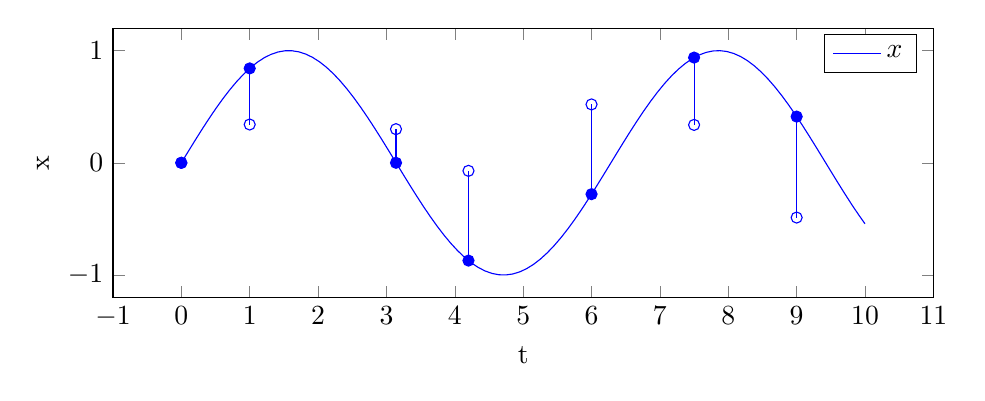
\begin{tikzpicture}
     \begin{axis}[width=12cm,height=5cm,xlabel=t,ylabel=x] 
     \addplot[blue,domain=0:10,samples=100]{sin(deg(x))};
     \addplot+[blue,draw=none,mark=*, mark options={blue},error bars/.cd, y dir=plus,y explicit,error mark=o,error mark options={blue,mark size=2pt}] 
     coordinates { 
      (0,0) +- (0,0) 
     (1,0.8415) +- (0.5,-0.5) 
     (3.14,0) +- (0.05,0.3) 
     (4.2,-0.8715) +- (0,0.8)
     (6.0,-0.27942) +- (0,0.8)
     (7.5,0.93799) +- (0.1,-0.6) 
     (9,0.41212) +- (0.3,-0.9)}; 
  \legend{$x$}
     \end{axis}
   \end{tikzpicture}
   \end{block}
\end{frame}



\begin{frame}[<+->]
  \frametitle{Datenassimilation Schritte}
	\begin{block}{Ziel: Minimiere Kostenfunktional}
	\begin{equation}\label{eq:costFunctional}
		\min_{x_o} J(x_0) = \min_{x_o} \frac{1}{2}\int_0^T \|Cx(t) - x_{Obs}(t)\|^2dt
	\end{equation}
	  $C$ - Projektion von $X_{\text{State}}$ nach $X_{\text{Obs}}$ 
	\end{block}
	\begin{block}{Datenassimilation Schritte}
	\begin{enumerate}
	 \item Berechnung Kostenfunktional
	 \item Berechnung $\nabla J(x_0)$
	 \item Optimierung
	\end{enumerate}
	\end{block}
\end{frame}
 
\begin{frame}[<+->]
  \frametitle{Datenassimilation Schritte}
  \begin{block}{Lösen einer ODE - z.B. Implizite Mittelpunktsregel(IMP)}
	\begin{equation}
	 x_n = x_a + h F \left(0.5 (x_a + x_n), t + 0.5 h\right)
	\end{equation}
	Speichere Werte $x_i$, berechne $J(x_0)$ mittels numerischer Quadratur
  \end{block}
  \begin{block}{Berechnung des Gradienten $\nabla J(x_0)$}
	Integriere das inhomogene adjungierte Tangent Linear Model rückwärts in $t$
	\begin{equation}
	  \dot{ \bar{x}}(t) =  -\frac{\partial F(x(t))}{\partial x}^\tr \bar x(t) +C^\tr(Cx(t) - x_{\text{obs}}(t)), ~ \bar x(T) =0
	\end{equation}
	\[
	\text{mit }\nabla J(x_0) = -\bar x(0)
	\]
  \end{block}
  \begin{block}{Optimierung}
	Optimiere $x_0$ mit einem geeigneten Verfahren über $J$ mit $\nabla J$ (z.B. BFGS)
  \end{block}

\end{frame} 

\begin{frame}[<+->]
  \frametitle{Problemstellung}
  \begin{block}{Problemstellung}
  \centering
	Wie kann die Datenassimilation für den Fall
	\[
	  \dot{x} = F(x),~ x_0 = x(0),~F\in C^{0,1}(\R^n)
	\]
	betrachtet werden?
  \end{block}
%   \begin{block}
   \begin{itemize}
    \item Unglatte Modelle in Ingeneursdisziplinen
    \item Elektrotechnik (Diode)
    \item Partielle Differentialgleichungen (Flux Limiter $\to$ Shallow Water Equation)
   \end{itemize}

%   \end{block}

\end{frame} 

\AtBeginSection[]
  {
     \begin{frame}<beamer>
%      \frametitle{Plan}
     \tableofcontents[currentsection]
     \end{frame}
  }
\section[Problemstellung]{Stückweise Linearisierung}
\begin{frame}[<+->]
\frametitle{Stückweise Linearisierung}
\begin{itemize}
\item Betrachte nun stückweise lineare Funktionen 
\[
\begin{aligned}
 f&:\R^n \to \R^m, \\
 f&\in \lbrace f_1,\ldots,f_k\rbrace,~f_i(x)=A_ix+b_i~\forall i,~f \text{ global stetig}
 \end{aligned}
\]
%  \item Betrachte nun $\dot{x} = F(x),~ x_0 = x(0),~F\in C^{0,1}(\R^n)$ (TODO stückweise lineare Funktionen ergänzen)
 \item $f$ ist als \textit{Abs Normal Form} darstellbar $\ldots$
 \end{itemize}
\begin{block}{Abs-Normal Form}
 \begin{equation}
\label{eq:absNormalForm}
  \begin{bmatrix}
   z\\y
  \end{bmatrix}
  =
  \begin{bmatrix}
   c\\b
  \end{bmatrix}
  +
  \begin{bmatrix}
   Z & L\\
   J & Y
  \end{bmatrix}
  \begin{bmatrix}
   x\\|z|
  \end{bmatrix}
 \end{equation}
wobei $c\in \R^s, ~ Z\in \R^{s\times n},~ L\in\R^{s\times s}, ~ b\in\R^m, ~ J\in\R^{m\times n}, ~ Y\in \R^{m\times s}$,\\
$s$ \textit{switching depth} und $z\in \R^s$ \textit{switching Variable}
\end{block}
\end{frame}

\begin{frame}[<+->]
\frametitle{Stückweise Linearisierung}
\begin{itemize}
 \item $\ldots$ und kann benutzt werden, um verkettet stückweise glatte Funktionen 
 \[
 \begin{aligned}
   f&:\R^n \to \R^m, \\
 f&\in \lbrace f_1,\ldots,f_k\rbrace,~f_i(x) \in C^1(\R^n)~\forall i,~f \text{ global stetig}\\
 &\text{verknüpft durch }\varphi_i \in \lbrace +,*,sin,exp,abs ,\ldots\rbrace                                                                
 \end{aligned}
 \]
an einer Entwicklungsstelle $\xo$ zu approximieren
%  \item Verkettet stückweise glatte Funktionen: stückweise definierte, stetige Funktionen, dessen Auswahlfunktionen stetig differenzierbar sind
% \item Diese Approximation heißt \textit{stückweise Lineariserung} an der Stelle $\xo$ und hat die Form 
% \[
%  F(\xo) + \Delta F(\xo; x-\xo)
% \]
% welche auch als \textit{tangent mode} bezeichnet wird.
\end{itemize}
% \begin{block}{Eigenschaften der Stückweisen Linearisierung}
%  \begin{itemize}
%   \item Blub
%   \item blob
%   \item Blubber
%  \end{itemize}
% \end{block}
\end{frame}

\begin{frame}[<+->]
\frametitle{Stückweise Linearisierung}
\begin{figure}
\centering
% \resizebox{.9\linewidth}{!}{ \documentclass{standalone}
\IfStandalone{
	\usepackage{pgfplots,pgfplotstable}
	\usetikzlibrary{external}
	\newcommand{\fromRoot}[1]{../#1}
	\newcommand{\D}{\Delta}
	\pgfplotsset{compat=1.9}
}{%
}

\begin{document}
\tikzsetnextfilename{piecewise_linearization}
\begin{tikzpicture}
\def\xo{-1};
\pgfmathdeclarefunction{f1}{1}{%
	\pgfmathparse{-(6/10)*(#1+2)^2}%
}
\pgfmathdeclarefunction{f2}{1}{%
	\pgfmathparse{3*( #1+sin((11/10)*deg(#1)) )}%
}
\pgfmathdeclarefunction{tf1}{1}{%
	\pgfmathparse{-1.2*(#1+1)-0.6}%
}
\pgfmathdeclarefunction{tf2}{1}{%
	\pgfmathparse{4.49687*(#1+1)-5.67362}%
}
\begin{axis}[
	height=0.45\textheight,
	axis y line = none,
	axis x line = bottom,
	xmin=-4,xmax=4,
	xtick = \empty,
	ytick = \empty,
	extra x ticks = {\xo},
	extra x tick labels={\(\mathring x\)},
	extra x tick style = {grid=major},
	domain=-4:4,
	samples=500,
]
\addplot[red!60!white] {f1(x)} 
	[yshift=2pt] 
	node[anchor=south,pos=0.8] {$F_1$};
\addplot[blue!60!white] {f2(x)} 
	node[anchor=south,pos=0.1] {$F_2$};
\addplot[black,yshift=1pt] {max(f1(x),f2(x)} 
	node[anchor=south,pos=0.2] {$F = \max(F_1,F_2)$};

\addplot[red!60!white,very thin] {tf1(x)} 
	node[anchor=south,pos=0.75,sloped] {$\mathring F_1 + F_1'(\mathring x)\D x$};
\addplot[blue!60!white,very thin] {tf2(x)} 
	node[anchor=north,pos=0.15,sloped] {$\mathring F_2 + F_2'(\mathring x)\D x$};
\addplot[black,very thin,yshift=1pt] {max(tf1(x),tf2(x)} 
	node[anchor=south,pos=0.75,sloped] {$\mathring F + \D F(\mathring x;\D x)$};
%\addplot [color=black,only marks,mark=*] coordinates { (-1,-0.6) };
%\addplot [color=black,only marks,mark=*] coordinates { (-1,-5.67362) };
\end{axis}
\end{tikzpicture}

 
\end{document}
 }
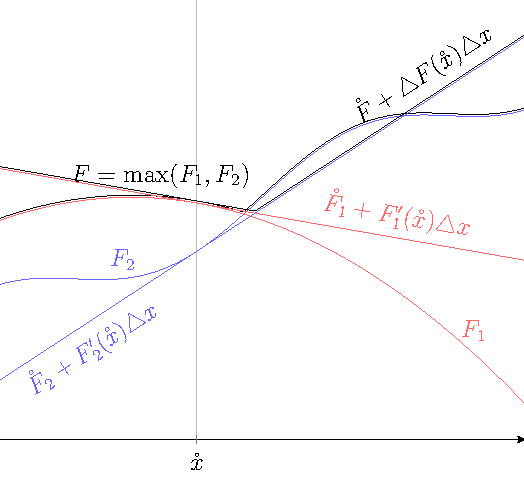
\includegraphics[width=0.65\linewidth]{../dipl_tex/img/tikz/piecewise_linearization.pdf}
\end{figure}
\end{frame}

\begin{frame}[<+->]
\frametitle{Stückweise Linearisierung}
\begin{block}{Eigenschaften}
 \begin{itemize}
  \item Inkrementfunktion 
    \[\Delta F(\xo;\Delta x) = F'(\xo;\Delta x)~ \text{für } \Delta x \leq \rho(\xo)\]
  \item Approximation 2. Ordnung: \[\|F(x) - F(\xo)- \Delta F(\xo;x-\xo)\| \leq \gamma \|x-\xo\|^2\]
 \end{itemize}
\end{block}
\begin{block}{AD}
 Automatische Berechnung der Stückweisen Linearisierung in Abs Normal Form mittels zusätzlicher AD Regel:
 \[
  \Delta v_i = (v_j \neq 0)?sign(v_j )\Delta v_j : abs(\Delta v_j) \text{ für } v_i = abs(vj), j\prec i
 \]
\end{block}

\end{frame}

\section[Problemstellung]{Verallgemeinerte implizite Mittelpunktsregel}
\begin{frame}[<+->]
\frametitle{Lösen von ODEs mittels stückweiser Linearisierung}
 \begin{block}{Verallgemeinerte implizite Mittelpunktsregel (GIMP)}
 \[
  x_n - x_a = h\int_{-\frac{1}{2}}^{\frac{1}{2}} F(\xo) + \Delta F(\xo; t(x-\xo))dt
 \]

\end{block}


\end{frame}

\section[Adjungierte Gleichung]{Adjungierte Gleichung}

\begin{frame}[<+->]
\frametitle{Berechnung von $\frac{\partial F(x)}{\partial x}$}
Nutze die erste Zeile der Abs Normal Form
\begin{align*}
z &= c+Zx + L\Sigma z \\
\iff (I-L\Sigma)z &= c+Zx  \\
\iff z &= (I-L\Sigma)^{-1}(c+Zx) 
\end{align*}
\pause
um sie in die zweite Zeile einzusetzen
\begin{align*}
y &= b+ Jx + Y|z| \\
\iff y &= b+ Jx + Y\Sigma z \\
\iff y &= b+ Jx + Y\Sigma (I-L\Sigma)^{-1}(c+Zx) \\
\iff y &= b+  Y\Sigma (I-L\Sigma)^{-1}c + \underbrace{(J + Y\Sigma (I-L\Sigma)^{-1}Z)}_{J_\sigma} x \\
\end{align*}
\vspace*{1cm}
wobei $(I-L\Sigma)^{-1} = I +L\Sigma + (L\Sigma)^2+\ldots$ eine Neumannreihe ist.
\end{frame}

\begin{frame}[<+->]
\frametitle{Differential Inclusion}
% GRADIENT NICHT NUR STETIGE UNGLÄTTEN SONDERN AUCH SPRÜNGE -> ABS EXAMPLE
\centering
\begin{figure}
  \begin{minipage}{0.45\textwidth} 
	\includegraphics[width=\linewidth]{../dipl_tex/img/tikz/adj_valley_tracing.pdf}
	\end{minipage}
	\hfill
	\begin{minipage}{0.45\textwidth}
	\includegraphics[width=\linewidth]{../dipl_tex/img/tikz/adj_valley_tracing1.pdf}	
	\end{minipage}
	
\end{figure}
Differential Inclusion und Valley Tracing Mode \\
\pause
Mögliche Lösungsansätze:\hfill
\begin{itemize}
 \item Polynomial Escape
 \item Einbeziehung der Kinks
\end{itemize}
\end{frame}
% \subsection{Polynomial Escape}
\begin{frame}[<+->]
\frametitle{Polynomial Escape}
\begin{block}{Polynomial Escape}
 Es kann kein Pfad der Form
 \[
  \Delta \hat x = \sum_{j=1}^n e_j t^j, ~ 0<t<\bar t, e_j\in R^n,~ \det(e_1,\ldots,e_n) \neq 0
 \]
für ein $\bar t$ auf einem Kink liegen (\cite[Proposition 6]{monster},\cite[S.11]{plan}).
%Nahc vorraussetzung gibts nur endlich viele hyperflächen (Kinks) -> darum geht das
\end{block}
\begin{block}{Firstsign}
 Nutze \[
        \firstsign(z_i,\Delta z_i^\tr \Delta x) =\sign (z_i + \Delta z_i)
       \]
wobei $\firstsign(z)$ das Signum des ersten nichtverschwindende Eintrag von $z$ ist, ansonsten 0.
\end{block}

\end{frame}
% \subsection{Adjungierte Gleichung}
\begin{frame}[<+->]
\frametitle{Adjungierte Gleichung}
\begin{figure}
\centering
\includegraphics[width=0.65\linewidth]{../dipl_tex/img/tikz/multiple_kinks_adjoint.pdf}
\end{figure}
\begin{figure}
\centering
% \resizebox{.9\linewidth}{!}{ \documentclass{standalone}
\IfStandalone{
	\usepackage{pgfplots,pgfplotstable}
	\usetikzlibrary{external}
	\newcommand{\fromRoot}[1]{../#1}
	\newcommand{\D}{\Delta}
	\pgfplotsset{compat=1.9}
}{%
}

\begin{document}
\tikzsetnextfilename{piecewise_linearization}
\begin{tikzpicture}
\def\xo{-1};
\pgfmathdeclarefunction{f1}{1}{%
	\pgfmathparse{-(6/10)*(#1+2)^2}%
}
\pgfmathdeclarefunction{f2}{1}{%
	\pgfmathparse{3*( #1+sin((11/10)*deg(#1)) )}%
}
\pgfmathdeclarefunction{tf1}{1}{%
	\pgfmathparse{-1.2*(#1+1)-0.6}%
}
\pgfmathdeclarefunction{tf2}{1}{%
	\pgfmathparse{4.49687*(#1+1)-5.67362}%
}
\begin{axis}[
	height=0.45\textheight,
	axis y line = none,
	axis x line = bottom,
	xmin=-4,xmax=4,
	xtick = \empty,
	ytick = \empty,
	extra x ticks = {\xo},
	extra x tick labels={\(\mathring x\)},
	extra x tick style = {grid=major},
	domain=-4:4,
	samples=500,
]
\addplot[red!60!white] {f1(x)} 
	[yshift=2pt] 
	node[anchor=south,pos=0.8] {$F_1$};
\addplot[blue!60!white] {f2(x)} 
	node[anchor=south,pos=0.1] {$F_2$};
\addplot[black,yshift=1pt] {max(f1(x),f2(x)} 
	node[anchor=south,pos=0.2] {$F = \max(F_1,F_2)$};

\addplot[red!60!white,very thin] {tf1(x)} 
	node[anchor=south,pos=0.75,sloped] {$\mathring F_1 + F_1'(\mathring x)\D x$};
\addplot[blue!60!white,very thin] {tf2(x)} 
	node[anchor=north,pos=0.15,sloped] {$\mathring F_2 + F_2'(\mathring x)\D x$};
\addplot[black,very thin,yshift=1pt] {max(tf1(x),tf2(x)} 
	node[anchor=south,pos=0.75,sloped] {$\mathring F + \D F(\mathring x;\D x)$};
%\addplot [color=black,only marks,mark=*] coordinates { (-1,-0.6) };
%\addplot [color=black,only marks,mark=*] coordinates { (-1,-5.67362) };
\end{axis}
\end{tikzpicture}

 
\end{document}
 }
\includegraphics[width=0.65\linewidth]{../dipl_tex/img/tikz/multiple_kinks_adjoint_new.pdf}
% \caption{Punkte $\xo$ der Gradientberechnung in der adjungierten Gleichung mit $\xo^{(i)} = \xo + 0.5(\tau_i+\tau_{i-1})\Delta x$}
\end{figure}
\centering
Gradientberechnung der adjungierten Gleichung mit $\xo^{(i)} = \xo + 0.5(\tau_i+\tau_{i-1})\Delta x$
\end{frame}

\begin{frame}[<+->]
\frametitle{Adjungierte Gleichung}
Wende auf die adjungierte Gleichung
\begin{align}
 \dot \xadj =  - \frac{\partial F(x;\Delta x)}{\partial x}^\tr \xadj + C^\tr (Cx-\xobs) 
\end{align}
\pause
die verallgemeinerte implizite Mittelpunktsregel an:
\begin{align}
%  \xadj_n -\xadj_a = \int_{-\frac{1}{2}}^{\frac{1}{2}}C^\tr
\xadj_n - \xadj_a &= h\cdot \int_{-0.5}^{0.5}C^\tr(C\xo-\rxobs) - \frac{\partial F(\xo,\Delta x)}{\partial x}^\tr \cdot \xadj dt\\
		  &= h\cdot \left[ C^\tr(C\xo-\rxobs) -\int_{-0.5}^{0.5} \frac{\partial F(\xo,\Delta x)}{\partial x}^\tr \cdot \xadj dt\right]
\end{align}
\pause
mit $N$ Kinks, $-0.5 = \tau_0 <\tau_1 <\ldots < \tau_N=0.5$ und $\mathring \tau_i = 0.5 (\tau_i +\tau_{i-1})$ folgt
\begin{align}
\xadj_n - \xadj_a &= h\left[ C^\tr(C\xo-\rxobs) - \sum_{i=1}^N \int_{\tau_{i-1}}^{\tau_{i}}\underbrace{\frac{\partial F(\xo+\mathring \tau_i\Delta x,\Delta x)}{\partial x}^\tr}_{A_i^\tr} \cdot \xadj dt\right]\\
\end{align}
\end{frame}

\begin{frame}[<+->]
\frametitle{Adjungierte Gleichung}
Mit  $\mathring \tau_i = 0.5 (\tau_i +\tau_{i-1})$ und $\Delta \tau_i = \tau_i-\tau_{i-1}$ folgt
\pause
\begin{align}
\xadj_n - \xadj_a &= h\cdot \left[C^\tr(C\xo -\rxobs) - \sum_{i=1}^N A_i^\tr \cdot \int_{\tau_{i-1}}^{\tau_{i}} \rxadj + t\Delta \xadj dt\right]\\
		  &= \ldots\\
		  &= h\cdot \left[C^\tr(C\xo -\rxobs) - \sum_{i=1}^N A_i^\tr \cdot \left( \diff \tau_i\cdot \rxadj +  \diff \tau_i \rtau_i \diff \xadj \right)\right]
\end{align}
\pause
Da $\rxadj = 0.5(\xadj_n + \xadj_a)$ und $\Delta \xadj = \xadj_n-\xadj_a$ gilt, folgt mittels Umsortieren
\[
\begin{aligned}
\left[I +h\sum_{i=1}^N A_i^\tr \left(\frac{1}{2} \diff \tau_i +\diff \tau_i \rtau_i\right) \right]\xadj_n &= 
&\left[I - h\sum_{i=1}^N A_i^\tr  \left(\frac{1}{2}\diff \tau_i-\diff \tau_i \rtau_i\right)\right]\xadj_a \\
&&+h C^\tr(C\xo -\rxobs)
\end{aligned}
\]
\end{frame}

% \subsection{Algorithmus}
% \begin{frame}[fragile]
% \frametitle{Algorithmus}
% \algrenewcommand{\algorithmiccomment}[1]{\hfill{\scriptsize #1}}
% \begin{algorithmic}[1]
%  \Function{calc\_kink\_partial}{$\cx,\hx,\Delta x$}
%  	\State $\hat{\tau} \gets 0$,$\check{\tau} \gets 0$, $x_{kink} \gets \cx$
%  	\State $\bar{A} \gets 0_{n\times n} $, $\hat{A} \gets 0_{n\times n}$
%  	\Repeat
%  	  \State $\check{\tau} \gets \check{\tau} + \hat{\tau}, ~ x_{kink} \gets x_{kink} +\check{\tau}\Delta x$
%  	  \State $\hat{\tau} \gets \check{\tau} + \Call{critMult}{ x_{kink},\Delta x}$ 		 \Comment{Berechne kritischen Multiplikator}
% 		\If{$\hat{\tau}>1$} $\hat{\tau}\gets 1$ \EndIf 
%  		\State $\xo \gets x_{kink}+0.5\cdot \hat{\tau} \Delta x$	\Comment{Berechne Mittelpunkt zwischen den Kinks}
%  	  \State $\frac{\partial F(\rx)}{\partial x} \gets $ gen\_jac($\rx,\Delta x$) \Comment{Berechne $\partial F$ aus der Abs-Normalform}
%  	  \State $\bar{A} \gets \bar{A} +  \frac{\partial F(\xo)}{\partial x} \cdot (\hat{\tau} - \check{\tau})$ 
%  		\State $\hat{A} \gets \hat{A} +  \frac{\partial F(\rx)}{\partial x} \cdot  \left(\frac{1}{2}(\check{\tau} + \hat{\tau})-0.5\right)$ \Comment{Verschiebe $\tau$ um $-0.5$}
%  \Until{$\hat{\tau} \geq 1$	}
%  \State \Return $[\bar{A}, \hat{A}]$;
%  \EndFunction
%  \end{algorithmic}
% \end{frame}
% 
% \begin{frame}[fragile]
% \frametitle{Algorithmus}
% \algrenewcommand{\algorithmiccomment}[1]{\hfill{\scriptsize #1}}
% \begin{algorithmic}[1]
% %  \Require $x_{0},t_0,T, h,x_{Obs}, TOL$
%  \Function{jac\_data\_assimilation}{$x_{0},t_0,T, h,x_{\text{obs}}, TOL$}
%  \State $N = \ceilS{\frac{t_0 - T}{h}}$, $\hat{\bar{x}} \gets 0$ \Comment{Setze Anfangswert}
%  \State $x \gets  \Call{solveODE}{x_0,t_0, T,h, TOL};$\Comment{Löse ODE in Vorwärtsrichtung}
%  \For{$k\gets$ N-1 to $1$} \Comment{Zeitschritt rückwärts}
%  	%\State $\rx \gets \cx - \frac h2 F(\cx)$ \Comment{initialization by half Euler}
%  	\State $\rx \gets 0.5(x_k + x_{k-1})$ \Comment{Berechne Mittelpunkt}
%  	\State $F(\rx) +\Delta F(\rx;\cdot) \gets$ \Call{Update}{} \Comment{Berechne neue Linearisierung an $\rx$}
%  	\State $\Delta x \gets x_{k-1}-x_k$\Comment{Berechne neue Richtung}
%  	\State $[\bar{A},\hat{A}] \gets \Call{calc\_kink\_partials}{x_k,x_{k-1},\Delta x}$  \Comment{Berechne $\partial F$}
%  	%\Until{$\|\hx - \cx - r - h F(\rx)\|$} < TOL
%  	\State{\begin{varwidth}[t]{\linewidth}$\check{\bar{x}} \gets$ Solve( \par
% 		    \hskip\algorithmicindent $I-\frac{h}{2}\bar{A}^\tr + h \hat{A}^\tr)\check{\bar{x}}=$\par 
% 		    \hskip\algorithmicindent $ (I+\frac{h}{2}\bar{A}^\tr + h\hat{A}^\tr)\hat{\bar{x}}- hC^\tr(C\rx-\rx_{\text{obs}}))$
% 		    \end{varwidth}
% 		    }
%  \EndFor
%  \State \Return $-\check{\bar{x}}$
%  \EndFunction
%   \end{algorithmic}
% \end{frame}

\chapter{Implementierung}
\section{Armadillo und OPENBlas}
Zur Implementierung der theoretischen Ergebnisse der letzten Kapitel wurde die C++ Klasse \textit{Armadillo} verwendet. 
Armadillo ist eine Template basierte C++ -Matrix-Vektor-Bibliothek, welche ähnliche Syntax wie Matlab zulässt. Neben Matrix-Matrix oder Matrix-Vektor Multiplikationen liefert sie eigene Lineare Gleichungssystemlöser mit, bietet einfache Möglichkeiten Teilmatrizen zu extrahieren und unterstützt teilweise Sparse Matrizen. Armadillo ist unter der Webseite \url{http://arma.sourceforge.net}(abgerufen am 26. November 2014) erreichbar und steht unter der \textit{Mozilla Public License 2.0} (\url{https://www.mozilla.org/MPL/2.0/}) als Open Source Projekt zur Verfügung.

Desweiteren unterstützt Armadillo Multi Threaded Operationen durch die Abstrahierung des OpenBlas Interfaces (\url{http://www.openblas.net/}, abgerufen am 26. November 2014), wodurch nahtlos Armadillos eigene Routinen durch die von OpenBlas ersetzt werden und trotzdem der Vorteil der einfachen Nutzbarkeit beibehalten bleibt. OpenBlas ist eine auf Parallelität optimierte Version der bekannten Linearen Algebra Bibliothek BLAS (Basic Linear Algebra Subprograms, \url{http://www.netlib.org/blas}). OpenBlas steht unter der BSD Lizenz (\url{http://www.linfo.org/bsdlicense.html}) zur Nutzung bereit.

\section{ADOL-C}
ADOL-C ist ebenfalls ein Open Source Bibliothek zur exakten automatischen Differentiation von C/C++ Programmen im Rahmen der Rechengenauigkeit. Im Mittelpunkt stehen dabei die \textit{aktiven Variablen}, welche die Initialisierungsvariablen darstellen. Diese werden mit einem eigenen Typ \texttt{adouble} initialisiert, welche eine Erweiterung der \texttt{double} Klasse darstellt. Mit diesen Werten wird die gewünschte Funktion, wie im Falle von \texttt{double}, zwischen den Aufrufen \texttt{trace\_on(tag)} und \texttt{trace\_off(tag)} ausgeführt und durch \textit{operator overloading} im gleichen Zug die Ableitung bestimmt. Intern erzeugt ADOL-C ein Tape, das den computational graph der Funktionsauswertung erstellt, auf welches durch \texttt{tag} referenziert wird. Nach dieser Auswertung bietet ADOL-C verschiedene Methoden dieses Tape auszuwerten.

ADOL-C wurde von Andreas Griewank erdacht und wird zurzeit in der Forschungsgruppe um Andrea Walther an der Universität Paderborn weiterentwickelt. Weitere Informationen zur Verwendung lassen sich in der Dokumentation \cite{walther2012getting} nachvollziehen. ADOL-C ist unter der \textit{Eclipse Public License 1.0} oder der \textit{GNU General Public License 2.0} in Projekten einsetzbar.

\section{Plan-C}
\label{sec:impl:planc}
Sämtliche Versuche wurden mit Plan-C erstellt. Plan-C ist eine C++ Bibliothek, welche im Rahmen der Diplomarbeit von Paul Boeck in \cite{boeck14} erarbeitet und dokumentiert wurde. Da im Rahmen der vorliegenden Arbeit rechenintensivere Beispiele betrachtet werden, wurde ein Fork dieser Bibliothek erstellt und Armadillo als Matrix - Vektor Bibliothek eingesetzt, um die allgemeine Performance zu steigern. Dies bedeutet, die in Boecks Arbeit als Verbesserungsvorschlag gegebene Benutzung von Sparse Matrizen einzubauen und mehrerer Prozessorkerne durch Parallelisierung zu unterstützen.  Desweiteren wurde die ursprüngliche Plan-C Klasse durch diverse Funktionen erweitert, damit sie die Datenassimilierung mittels stückweiser Linearisierung unterstützt. Eine kurze Dokumentation der wichtigsten Funktionen soll im Folgenden dargelegt werden. Das Interface zu Plan-C ist im Anhang \ref{sec:source} beschrieben.

\subsection{Abs-Normal Form}
Plan-C ist eine C++ Klasse, die ein Objekt zur Verfügung stellt, welche eine Abstraktion einer Funktion darstellt. Intern wird der Reverse Mode von \texttt{ADOL-C} benutzt, um zu einer gegebene Funktion die Abs-Normal Form an einem gegebenen Entwicklungspunkt aufzustellen und mit ihr zu rechnen.

Um ein Plan-C Objekt zu erstellen kann man entweder direkt die Abs-Normal Form mit den Matrizen aus Gleichung  \eqref{eq:absNormalForm} 
\begin{lstlisting}
 PlanC(vec c,vec b,mat Z, mat L, mat J, mat Y, vec xo);
\end{lstlisting}
oder eine Funktion \texttt{func} übergeben
\begin{lstlisting}
 PlanC(size_t n,size_t m,vec xo, simple_function func, short tag);
\end{lstlisting}
\texttt{vec} und \texttt{mat} sind die Armadillo internen Klassen für Vektoren bzw. Matrizen, während \texttt{n} und \texttt{m} die Dimensionen des Definitions-/Werteberech der Funktion \texttt{func} und \texttt{xo} den Entwicklungspunkt beschreibt. \texttt{tag} gibt an, welches Tape von \texttt{ADOL-C} benutzt werden soll. 
Die Funktion \texttt{func} muss in der Form 
\begin{lstlisting}
 void (simple_function*) (short tag, double* px, double* py);
\end{lstlisting}
initialisiert werden, damit \texttt{Plan-C} diese verarbeiten kann. \texttt{tag} ist wieder die Nummer des benutzten Tapes,  \texttt{px} ein Pointer auf die Eingabeparameter und \texttt{py} beschreibt die Rückgabewerte. 
Beispielsweise ist eine Funktion gegeben als
\begin{lstlisting}[caption=Beispiel einer simple\_function,label=lst:simpleFunc]
 void func(short tag, double* px, double* py){
 //aktiviere Abs Normal Form Berechnung
  enableMinMaxUsingAbs();
  //beginne Taping auf tag
  trace_on(tag);
  size_t n = 2;
  size_t m = 2;
  x = new adouble[n];
  y = new adouble[m];
  for(size_t i=0;i<n;i++){
    //markiere fuer alle i x[i] als aktive Variable
    x[i] = <<= px[i]		
  }
  
  //Fuehre Berechnungen durch
  y[0] = fabs(x[0]+x[1]);
  y[1] = x[0] + fabs(x[0]-x[1]);
  
  for(size_t i=0;i<m;i++){
    //markiere y[i] als Resultat
    y[i] = <<= px[i]		
  }
  delete[] x, delete[] y;
  // stoppe taping
  trace_off(tag); 
 }
\end{lstlisting}

Die Methoden \texttt{enableMinMaxUsingAbs}, \texttt{trace\_on} und \texttt{trace\_off} sind \texttt{ADOL-C} interne Funktionen, wobei \texttt{enableMinMaxUsingAbs} erst im Rahmen der Entwicklung von \texttt{Plan-C} zu \texttt{ADOL-C} hinzugefügt wurde. Alle arithmetischen Operatoren der \texttt{std::cmath} Klasse wurden von \texttt{ADOL-C} überladen.

In \texttt{Plan-C} werden im Konstruktor folgende Methoden benutzt
\begin{description}
 \item[\texttt{get\_num\_switches}] gibt die Menge der switching Variablen zurück
 \item[\texttt{zos\_an\_forward}] Analysiert das Tape und behält Ableitungen erster Ordnung, berechnet \texttt{z}
 \item[\texttt{fos\_an\_reverse}] Die Matrizen \texttt{Z,L,Y} und \texttt{J} werden aus dem Tape errechnet und zeilenweise zurückgegeben
\end{description}
Mithilfe dieser drei Funktionen wird die Abs-Normal Form als Matrix-Repräsentation aufgestellt.
Desweiteren stellt das \texttt{Plan-C} Objekt weitere Funktionen zur Verfügung:
\begin{description}
 \item[\texttt{update\_linearization(vec xo)}] Berechnet die Abs-Normal Form an der Stelle \texttt{xo}
 \item[\texttt{eval(vec x)}] Wertet die Abs-Normal Form an Stelle \texttt{x} aus
 \item[\texttt{eval\_F(vec x)}] Wertet die Ausgangsfunktion an Stelle \texttt{x} aus 
\end{description}

\subsection{Verallgemeinerte Mittelpunktsregel}
Die Implementierung der verallgemeinerten Mittelpunktregel in C++ wird analog dem Pseudocode aus Prozedur \ref{alg:genMidpointRule} programmiert. Eingangsparameter ist ein Vektor der zeitdiskretisierten Zeitachse \texttt{t} und der Anfangswert \texttt{x0}. Zusätzlich kann man eine \texttt{verbose} Flag übergeben, welche mehr Log-Ausgaben zur Konsequenz hat, sowie den Toleranz Parameter \texttt{TOL}. Zurückgegeben wird die Lösung in Form einer Matrix \texttt{x}, wobei die Zeile \texttt{x.row(i)} zur Stützstelle \texttt{t(i)} gehört.
\begin{lstlisting}[caption=Verallgemeinerte Mittelpunktsregel,label=lst:genMidpointRule]
 mat PlanC::solve_ode(const vec &t, const vec &x0, bool verbose, double TOL) {
  size_t N = t.n_elem;
  //setze Anfangswert
  x.row(idx) = x0.t();
  ...
  //Initialisierung der Vektoren
  ...	
  while (idx < N - 1) {
    ++idx;
    //berechne Schrittweite
    h= fabs(t(idx)-t(idx-1));
    //Initialschritt mit halben Euler
    xo = xc + h * 0.5 * eval_F(xc);		
    do {
      ... 
      ++cnt_inner_it;
      //erstellt ein Update der Abs-Normal Form an Punkt xo
      updateLinearization(xo);
      v = 2.0 * (xo - xc);
      //Berechne Residuum
      r = h * (integrate(v) + integrate(-v) - fxo);
      PlanC tmp = scale_shift(2.0, -h);
      //Loese LGS mittels PL-Newton
      xo = tmp.solve(r + 2.0 * xc, false, 1E-14);
      res = 2.0 * xo - 2.0 * xc - r - h * eval_F(xo);
      //Berechne Euklidische Norm des Fehlers
      resError = arma::norm(res);
      ...
    } while (resError > TOL && cnt_inner_it < MAX_IT);
    if (cnt_inner_it == MAX_IT) {...}//error
    xc = 2 * xo - xc;    
    x.row(idx) = xc.t();
  }
  return x;
}
\end{lstlisting}
Die Methode \texttt{integrate} ist die Implementierung der Prozedur \ref{alg:quad} und \texttt{scale\_shift} erstellt eine verschobenes \texttt{Plan-C} Objekt, welches für die stückweise lineare Newton Prozedur \ref{eq:unfoldedNewton} verwendet wird.
\subsection{Berechnung des Kostenfunktionals}\label{sec:implementation:costfunctional}
% \subsection{Projektionsoperator}
Die Berechnung des Kostenfunktionals \eqref{eq:costfunctional} ist prinzipiell die Berechnung der $L^2$- Norm der Differenz der Observierungsparameter mit den errechneten Werten. Zur Implementierung wird zuerst die Lösung des Systems an der Stelle \texttt{x0} errechnet und danach mittels der Trapezregel die $L^2$-Norm berechnet. Die Trapezregel 
\[
 T_i(f) = h_i \frac{f(x_{i+1})+f(x_i)}{2}
\]
mit $h_i = t_{i}-t_{i-1}$ und $i=1,\ldots,n-1$ lässt sich für mehrere Stützstellen zusammenfassen zu
\[
 T(f) =\frac{1}{2} \left(h_1 f(x_0) + h_{n-1} f(x_{n-1}) + \sum_{i=1}^{n-2} f(x_i)(h_i+h_{i+1})\right)
\]
Daraus ergibt sich analog der Algorithmus \ref{lst:costFunctionalAlg}. Die Eingabeparameter wird zum einen der Vektor \texttt{tState} übergeben, welcher die Stützstellen des ODE Lösers beschreibt, \texttt{xo} ist der auszuwertende Punkt, \texttt{tObs} die Stützstellen der Observierung, \texttt{xObs} die Observierungsparameter und die \texttt{verbose} Flag.
\begin{lstlisting}[caption=Berechnung des Kostenfunktionals,label=lst:costFunctionalAlg]
double PlanC::cost_functional_data_assimilation(const vec &tState, const vec &x0, const vec &tObs, const mat &xObs, bool verbose) {
  size_t N = tState.n_elem;
  double t_a = tState(0);
  ...
  //Projektion der Loesung in den Raum der Observierungsparameter
  xState = solve_ode(tState, x0, verbose, TOL);
  xCalc = projState2ObsSpline(tState, tObs,xState);
  
  size_t NObs = tObs.n_elem;
  double Jac = 0.0;
  Jac += fabs((tObs(1) - tObs(0))) * pow(arma::norm(xCalc.row(0) - xObs.row(0)),2);
  Jac += fabs((tObs(NObs-1) - tObs(NObs-2))) * pow(arma::norm(xCalc(NObs-1) - xObs(NObs-1)),2);

  for (size_t i = 1; i < NObs - 1; i++) {
    hi = fabs((tState(i) - tState(i-1)));
    //Trapezregel
    Jac += hi*pow(fabs(xCalc(i)- xObs(i)),2);
  }
  return 0.5 * 0.5*Jac;
}
\end{lstlisting}
Die Methode \texttt{projState2ObsSpline} erstellt eine Spline Interpolation der Lösung \texttt{xState} und projeziert die interpolierten Werte auf die Stützstellen \texttt{tObs} des Observierungsraumes. In Gleichung \eqref{eq:costfunctional} ist dies identisch mit dem Projektionsoperator $C$. Falls \texttt{tObs} eine Teilmenge von \texttt{tState} ist, so ist $C$ tatsächlich eine Matrix. In dieser Arbeit ist die Anzahl der Stützstellen von \texttt{tState} immer größer oder gleich der Anzahl der Stellen der Observierungsparameter \texttt{tObs}. Denkbar wären auch der umgedrehte Fall.

\subsection{Adjungierte Mittelpunktsregel}
Die Implementierung der adjungierten Mittelpunktsregel wird analog zu Algorithmus \ref{alg:jacDataAssimilation} durchgeführt. Eingabeparameter sind der Stützstellenvektor \texttt{tState}, der Entwicklungspunkt \texttt{x0}, die Observierungsparameterstützstellen \texttt{tObs}, die Observierungsparameter \texttt{xObs}, die Toleranz zur Lösung der ODE \texttt{TOL} und die \texttt{verbose} Flag.
\begin{lstlisting}[caption=Berechnung der adjungierten Mittelpunktsregel, label=lst:adjMidpointRule]
vec PlanC::jac_data_assimilation_pl(const vec &tState, const vec &x0, const vec &tObs, const mat &xObs,double TOL, bool verbose) {
  size_t N = tState.n_elem;
  double h = fabs(tState(1)-tState(0));
  double t_end = tState(tState.n_elem - 1) + h;

  //1. Schritt: Loese ODE
  mat xCalc = solve_ode(tState, x0, verbose, TOL,xoForward);
  
  //2. Schritt: Hin und Rueckprojektion
  mat xCalcProjInObs = projState2ObsSpline(tState, tObs, xCalc) - xObs;
  mat xCalcProj = projObs2StateSpline(tState, tObs, xCalcProjInObs);
  
  //3. Schritt: Loese Adj TLM Rueckwaerts in der Zeit
  int idx = N - 1;
  
  vec xc(n,fill::zeros); //Nullvektor als Anfangsbedingung
  vec xCalcO(n);	 //Mittelpunkt
  vec xCalcMinusXObsProj(n); //Differenz xObs zu xCalc 
  mat A(n, n);
  vec b(n);
  sp_mat I = speye<sp_mat>(n,n);//Identitaetsmatrix
  while (idx > 0) {
    mat ABar(n, n,fill::zeros);
    mat AHat(n, n,fill::zeros);
    //Berechne Richtung
    d = (xCalc.row(idx - 1) - xCalc.row(idx)).t();
    //Berechne Mittelpunkt
    xCalcO = 0.5 * 
	(xCalc.row(idx) + xCalc.row(idx - 1)).t();
    xCalcMinusXObsProj = 0.5 * 
	  (xCalcProj.row(idx) + xCalcProj.row(idx - 1)).t();
    //Erstelle neue AbsNormal Form am Mittelpunkt xCalcO
    updateLinearization(xCalcO);
    
    //Berechne gewichtete Ableitung
    calc_kink_partial(
	  xCalc.row(idx).t(), 
	  xCalc.row(idx - 1).t(),
	  d,
	  ABar,
	  AHat
    );
    A = I - 0.5 * h * ABar + h * AHat;
    b = (I + 0.5 * h * ABar + h * AHat) * xc - h * (xCalcMinusXObsProj);
    xc = arma::solve(A, b);
    idx = idx - 1;
  }
  return (-1) * xc;
}
\end{lstlisting}
Die Funktion \texttt{calc\_kink\_partial} spiegelt genau den Algorithmus \ref{alg:kinkPartials} wider.
\begin{lstlisting}[caption=Berechnung der gewichteten Ableitung, label=lst:kinkPartials]
void PlanC::calc_kink_partial(vec xCheck, vec xHat,const vec &d, mat &A, mat &B) {
  vec xKink = xCheck;
  double tau(0), tau_old(0),deltaTau, rTau;
  do {
    //Kritischer Multiplikator
    tau =  crit_mult(xKink,d,1);
    tau = tau+tau_old;
    //Inkrement zum naechsten Kink
    dx = tau * d;
    deltaTau = tau - tau_old;
    //Shifte Interval von [0,1] nach [-0.5,0.5]
    rTau = 0.5 * (tau + tau_old)-0.5;
    //Ableitung an der Stelle xKink
    df = gen_jac(xKink, dx, true).t();
    //Gehe zum naechsten Kink
    xKink = xKink + dx;

    A += df * deltaTau;
    B += df * deltaTau * rTau;
    tau_old = tau;
  } while (tau < 1);
}
\end{lstlisting}

Die Methode \texttt{gen\_jac(vec x,vec d,bool disableKinkPrediction)} berechnet den zum jeweiligen Polyeder zugehörige limiting Jacobian an Stelle \texttt{x} in Richtung \texttt{d} mittels des Polynomial Escape Algorithmus 
% \ref{alg:genjac}
\ref{alg:polynomialEscape}
. Die Flag \texttt{disableKinkPrediction} ist gesetzt, damit nicht noch einmal das nächste $\tau$ berechnet wird.


\subsection{Optimierung}
Die Optimierungsmethode ist ebenfalls im \texttt{PlanC} Objekt untergebracht. Sie berechnet nun mittels BFGS Verfahren \ref{alg:bfgs} mit Wolfe-Powell Linesearch \ref{alg:wolfePowell} das Minimum. 
Als zu minimierende Funktion wird die Methode \texttt{cost\_functional\_data\_assimilation} verwendet und als erste Ableitung die Prozedur \texttt{jac\_data\_assimilation\_pl}.

% \begin{lstlisting}
% solve_data_assimilation_bfgs
% (vec &tState, vec &x0,vec &tObs, mat &xObs, mat &weights, double TOL,
% 		mat &iterationSteps, bool verbose, int type) 
% \end{lstlisting}
% 

\chapter{Experimente}
In diesem Kapitel werden wir drei verschiedenen Beispielen mit sämtliche eingeführten Methoden duchrechnen. Dabei wird zunächst auf die Lösung der Differentialgleichung eingegangen und Konvergenzbetrachtungen durchgeführt. Danach wird der Gradienten des Kostenfunktionals behandelt und die Optimierung für diverse Anfangswerte durchgeführt. %Stay Tuned!
\section{Rolling Stone}
% \subsection{Problemstellung}
Zum Anfang wollen wir uns dem sogenannten Rolling Stones Beispiel widmen, welches beispielsweise in \cite{boeck2014experiments} oder \cite{hasenfelder13} behandelt wurde. 
Es behandelt eine sich reibungslos bewegende Kugel auf einer konvexen Parabel, in dessen Mitte eine flache Ebene auf dem Intervall $[-1,1]$ eingefügt wurde. 
\begin{figure}[ht]
\centering
\begin{minipage}[b]{0.49\linewidth}
% \begin{minipage}[t][3cm][t]{5cm}
\documentclass{standalone}
\IfStandalone{
	\usepackage{pgfplots,pgfplotstable}
	\usetikzlibrary{external}
	
	}{%
}
% \usepackage{pgfplots,pgfplotstable}
% \usetikzlibrary{external}
	

\begin{document}
\tikzsetnextfilename{rolling-stones}
\begin{tikzpicture}[x=3em,y=3em]
\begin{axis}[
            xmin=-2.5,xmax=2.5,
            ymin=-1.5,ymax=1.5,
            xlabel=$z$,
%             legend entries={$V(z)$,$V'(z)$},
            width=\linewidth
        ]
        \addplot[domain=-2.5:-1]{(1+x)^2/2};
        \addplot[-,domain=-1:1]{0};
        \addplot[domain=1:2.5]{(1-x)^2/2};
        \addplot[domain=-2.5:2.5,samples=100,blue]{-min(max(-1-x,0),1-x)};
\end{axis}
\end{tikzpicture}

 
\end{document}

\caption{Rolling Stones}
\label{fig:rollingStones}
\end{minipage}
% \quad
\begin{minipage}[b]{0.49\linewidth}
% \begin{minipage}[t][3cm][t]{5cm}
\documentclass{standalone}
\IfStandalone{
	\usepackage{pgfplots,pgfplotstable}
	\usetikzlibrary{external}
	
	}{%
}
\begin{document}
\tikzsetnextfilename{rolling-stones-solution}
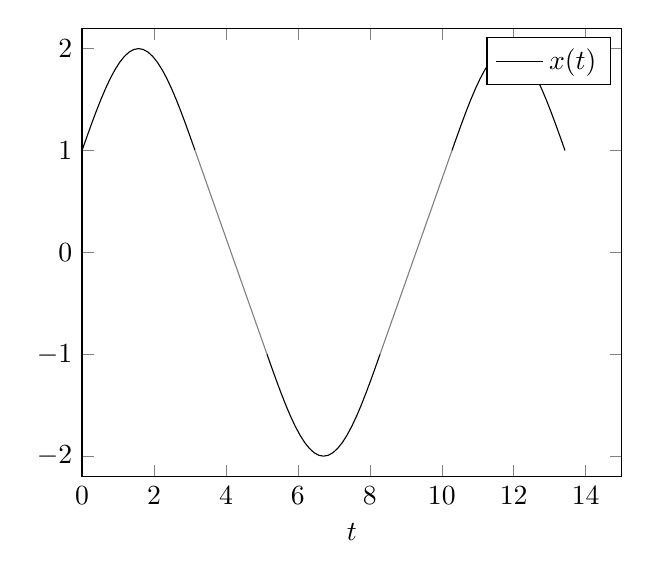
\begin{tikzpicture}[x=3em,y=3em]
\begin{axis}[
            xmin=0,xmax=15,
            ymin=-2.2,ymax=2.2,
            xlabel=$t$,
            legend entries={$x(t)$}
        ]
        \addplot[domain=0:3.14]{1+sin(deg(x))};
        \addplot[domain=pi:pi+2,gray]{1-x+pi};
        \addplot[domain=pi+2:2*pi+2]{-1-sin(deg(2-x))};
        \addplot[domain=2*pi+2:2*pi+4,gray]{x-3-2*pi};
        \addplot[domain=2*pi+4:3*pi+4]{1+sin(deg(x-2*pi-4))};
\end{axis}
\end{tikzpicture} 
\end{document}

\caption{Rolling Stones Lösung}
\label{fig:rollingStonesSolution}
\end{minipage}
\end{figure}
Figur \ref{fig:rollingStones} zeigt die Rampe
\[
 V(z) = \left(\frac{(1+z)^2}{2}\right)\chi_{(-\infty,-1]} + \left(\frac{(1-z)^2}{2}\right)\chi_{[1,\infty)} ,
 ~ \chi_{[a,b)}(z) = 
 \begin{cases}
  1 & z \in [a,b)\\
  0 & \text{sonst}
 \end{cases}
\]

und deren Ableitung, welche wir als gewöhnliche Differentialgleichung
 \begin{equation}
  \begin{pmatrix}
   \dot x_1 \\
   \dot x_2 \\
  \end{pmatrix}
 = 
 \begin{pmatrix}
  x_2 \\
  -x_1 - \frac{|x_1-1|}{2} + \frac{|x_1+1|}{2}
 \end{pmatrix}
=F(x)
\label{eq:rolling_stones}
 \end{equation}
auffassen, wobei $x_1$ die Abszissenposition des Steines und $x_2$ dessen Geschwindigkeit bezeichnet.
Die Funktion \eqref{eq:rolling_stones} ist stückweise linear, sodass wir seine Abs Normal Form \eqref{eq:absNormalForm} angeben können mit
\[
c = \begin{pmatrix}
     -1\\
     1
    \end{pmatrix}
\quad
 Z = \begin{pmatrix}
      1 & 0 \\
      1 & 0
     \end{pmatrix}\quad
J = \begin{pmatrix}
      0&1\\
      -1 & 0
     \end{pmatrix}\quad
 Y = \begin{pmatrix}
      0 & 0\\
      -0.5  & 0.5
     \end{pmatrix}
\]
der Rest wird passend zur Dimension zu $0$ gesetzt. Für das Rolling Stones Beispiel lässt sich eine analytische Lösung zur ODE \eqref{eq:rolling_stones} für den Anfangswert $x_0=(1,1)$ angeben. Sie ist $2\pi+4$ periodisch, hat die Form
\begin{equation}
 x(t) = \begin{cases}
         1+\sin(t) 	& 0\leq t \leq \pi	\\
         1-(t-\pi) 	& \pi \leq t < \pi+2	\\ 
         -1 - \sin(2-t) 	& \pi+2\leq t<2\pi+2	\\
         t-3-2\pi	& 2\pi+2 \leq t<2\pi +4
        \end{cases}
\label{eq:analyticSolRolling}
\end{equation}
und wird in Figur \ref{fig:rollingStonesSolution} angegeben. Dabei sind die grau eingezeichneten Bereiche linear.

\subsection{Lösen der ODE}
% Die Konvergenz der verallgemeinerten impliziten Mittelpunktsregel 
\begin{figure}
\centering
\documentclass{standalone}
\IfStandalone{
	\usepackage{pgfplots,pgfplotstable}
	\usetikzlibrary{external}
	\newcommand{\fromRoot}[1]{../#1}
}{%
}
\begin{document}
\tikzsetnextfilename{convergence_rolling_plot}
\begin{tikzpicture}
\begin{loglogaxis}[
	width=10cm,
	xlabel=Degrees of freedom $N$,
	ylabel=Error at time $T$,
	legend entries ={Expl. MP,
	IMP,
	GIMP, 
	}
]
  	\addplot[mark=none,red,very thin] table[x index=0,y index=2] {img/data/convergence_rolling_plot.dat};%expl midpoint
 	\addplot[mark=none,green,very thin] table[x index=0,y index=3] {img/data/convergence_rolling_plot.dat};%impl midpoint
	\addplot[mark=none,blue,very thin] table[x index=0,y index=1] {img/data/convergence_rolling_plot.dat};%gen midpoint

	\addplot[mark=none,very thin,gray, yshift=-20pt] 
		table[y={create col/linear regression={x=0,y=1}}] {img/data/convergence_rolling_plot.dat}
		  coordinate [pos=0.5] (A)
		  coordinate [pos=0.6] (B)
		;
	% save the slope parameter:
	\pgfmathparse{-\pgfplotstableregressiona}	
	\pgfmathsetmacro{\slope}{\pgfmathresult}
	
	% draw the opposite and adjacent sides
	% of the triangle
	\draw[very thin,gray] (B) -| (A)
	node [pos=0.2,anchor=north]
	{\pgfmathprintnumber{\slope}};
\end{loglogaxis}
\end{tikzpicture}
\end{document}
\caption{Konvergenz Rolling Stones im Intervall $[0,50]$ mit $x_0=(1,1)$}
\label{fig:rollingStonesConvergence}
\end{figure}


\begin{figure}[H]
\footnotesize 
\centering
% \quad
\begin{minipage}[b]{0.45\linewidth}
% \begin{minipage}[t][3cm][t]{5cm}
\documentclass{standalone}
\IfStandalone{
	\usepackage{pgfplots,pgfplotstable}
	\usetikzlibrary{external}
	\newcommand{\fromRoot}[1]{../#1}
}{%
}

\begin{document}
\tikzsetnextfilename{rolling_energy_error}
\begin{tikzpicture}
\begin{loglogaxis}[
	width=\linewidth,
	xlabel=Anzahl der Freiheitsgrade $N$,
	ylabel=Mittelwert des Energieverlustes,
	legend entries ={Expl. MP,
	IMP,
	GIMP 
	},
	legend style={at={(0.5,1.0)},anchor=south},
	legend columns=2
]
  	\addplot[mark=none,red,very thin] table[x index=0,y index=2] {\fromRoot img/data/rolling_energy_error.dat};%expl midpoint
 	\addplot[mark=none,green,very thin] table[x index=0,y index=3] {\fromRoot img/data/rolling_energy_error.dat};%impl midpoint
	\addplot[mark=none,blue,very thin] table[x index=0,y index=1] {\fromRoot img/data/rolling_energy_error.dat};%gen midpoint
\end{loglogaxis}
\end{tikzpicture}
\end{document}
\caption{Rolling Stones Energieverlust im Intervall $[0,2\pi+4]$ mit $x_0=(1,1)$}
\label{fig:rollingStonesEnergyError}
\end{minipage}
\quad
\begin{minipage}[b]{0.45\linewidth}
% \begin{minipage}[t][3cm][t]{5cm}
\documentclass{standalone}
\IfStandalone{
	\usepackage{pgfplots,pgfplotstable}
	\usetikzlibrary{external}
	\newcommand{\fromRoot}[1]{../#1}
}{%
}
\begin{document}
\tikzsetnextfilename{convergence_rolling_romberg_plot}
\begin{tikzpicture}
\begin{loglogaxis}[
	width=10cm,
	xlabel=Anzahl der Freiheitsgrade $N$,
	ylabel=Fehler in $x$,
% 	title=Convergence of SWE,
	legend entries ={
% 	Expl. MP,
	IMP,
	GIMP, 
	Romberg Impl,
	Romberg Gen
	}
]
 	\addplot[mark=none,green,very thin] table[x index=0,y index=3] {img/data/convergence_rolling_romberg_plot.dat};%impl midpoint
	\addplot[mark=none,blue,very thin] table[x index=0,y index=1] {img/data/convergence_rolling_romberg_plot.dat};%gen midpoint

	\addplot[mark=none,lime,very thin] table[x index=0,y index=5] {img/data/convergence_rolling_romberg_plot.dat};%Romberg impl midpoint
	\addplot[mark=none,cyan,very thin] table[x index=0,y index=4] {img/data/convergence_rolling_romberg_plot.dat};%ROMBERG gen midpoint
	
	
	\addplot[mark=none,very thin,gray, yshift=-20pt] 
		table[y={create col/linear regression={x=0,y=4}}] {img/data/convergence_rolling_romberg_plot.dat}
		  coordinate [pos=0.5] (A)
		  coordinate [pos=0.6] (B)
		;
	% save the slope parameter:
	\pgfmathparse{-\pgfplotstableregressiona}	
	\pgfmathsetmacro{\slope}{\pgfmathresult}
	
	% draw the opposite and adjacent sides
	% of the triangle
	\draw[very thin,gray] (B) -| (A)
	node [pos=0.2,anchor=north]
	{\pgfmathprintnumber{\slope}};
\end{loglogaxis}
\end{tikzpicture}
\end{document}
\caption{Konvergenz der Romberg Extrapolation im Intervall $[0,50]$ mit $x_0=(1,1)$}
\label{fig:rollingStonesConvergenceRomberg}
\end{minipage}

\end{figure}


Die in Theorem \ref{thm:convergenceGenMidpoint} vorhergesagte Konvergenzordnung von $\mathcal O(h^2)$ erfüllt die verallgemeinerte implizite Mittelpunktsregel wie in Figur \ref{fig:rollingStonesConvergence} ersichtlich.
Dass die gewöhnliche implizite Mittelpunktsregel eine ebenso hohe Konvergenzrate besitzt ist darin begründet, dass sie im gegebenen Intervall nur $4$ mal pro $2\pi+4$ Periode Unglattheiten überquert, sonst jedoch normal konvergiert. Aufgrund dieser Unglattheiten entsteht für die implizite Mittelpunktsregel (IMP) kein glatter Konvergenzgraph, sondern sie springt. Demgegenüber konvergiert die verallgemeinerter implizite Mittelpunktsregel (GIMP) sehr stabil, da sie die Knicke der Funktion mit in ihre Berechnung einbezieht.
Insbesondere wird der Fehler der GIMP mit zunehmender Zeit (siehe Fig. \ref{fig:rollingStonesEOT}) nur in den nicht affinen Abschnitten größer während in den affinen Abschnitten exakt gelöst wird, der lokale Fehler der IMP erhöht sich jedoch ständig, bedingt durch die Kinks und der zu großen Schrittweite. Der allgemeine Fehler ist dadurch für die IMP höher über die Zeit gesehen als der Fehler der GIMP (\ref{fig:rollingStonesEOT}(b)).

Da sich der rollende Stein reibungslos in unserem System bewegt, muss die analytische Lösung die komplette Energie erhalten, d.h. die potentielle Energie addiert mit der kinetischen $V(x) + \frac{1}{2}\dot x^2$ muss konstant sein. Das Bild \ref{fig:rollingStonesEnergyError} wurde mittels der summierten Variation der Energie 
\begin{equation}
 h \left[\sum_{l=0}^{T/h} \left( V(x_1^l) + \frac{1}{2} (x_2^l)^2 -\frac{1}{2}\right)^2\right]^{\sfrac{1}{2}}
 \label{eq:energyVariation}
\end{equation}
berechnet. Es ist deutlich zu erkennen, dass die Energie mit der GIMP deutlich besser erhalten bleibt als mit den klassischen Methoden, selbst für große Schrittweiten.
Dadurch führt die in Figur \ref{fig:rollingStonesConvergenceRomberg} durchgeführte Romberg Extrapolation zu sehr guten Ergebnissen. Da der Konvergenzgraph der GIMP stabil ist, lässt sich eine gute Extrapolation mit Konvergenzen der Ordnung 3 bis 4 erreichen. Demgegebenüber besitzt die Extrapolation der IMP keine höhere Konvergenzordnung als die der IMP selbst.
\begin{figure}[H]
\footnotesize 
\centering
\begin{minipage}[b]{0.49\linewidth}
% \begin{minipage}[t][3cm][t]{5cm}
\documentclass{standalone}
\IfStandalone{
	\usepackage{pgfplots,pgfplotstable}
	\usetikzlibrary{external}
	\newcommand{\fromRoot}[1]{../#1}
}{%
}
\begin{document}
\tikzsetnextfilename{rolling_error_over_time}
\begin{tikzpicture}
\begin{axis}[
	width=\linewidth,
	xlabel=Zeitpunkt $t$,
	ylabel=Fehler zum Zeitpunkt $t$,
	legend entries ={Expl. MP,
	IMP,
	GIMP, 
	},
	legend style={at={(0,1)},anchor=north west}
]
\addplot[mark=none,red,very thin] table[x index=0,y index=3] {img/data/rolling_error_over_time.dat};
\addplot[mark=none,green,very thin] table[x index=0,y index=2] {img/data/rolling_error_over_time.dat};
\addplot[mark=none,blue,very thin] table[x index=0,y index=1] {img/data/rolling_error_over_time.dat};

\end{axis}
\end{tikzpicture}
\end{document}
\caption*{(a) Am Zeitpunkt $t$}\end{minipage}
% \quad
\begin{minipage}[b]{0.49\linewidth}
% \begin{minipage}[t][3cm][t]{5cm}
\documentclass{standalone}
\IfStandalone{
	\usepackage{pgfplots,pgfplotstable}
	\usetikzlibrary{external}
	\newcommand{\fromRoot}[1]{../#1}
}{%
}
\begin{document}
\tikzsetnextfilename{rolling_error_over_time_all}
\begin{tikzpicture}
\begin{axis}[
	width=\linewidth,
	xlabel=Zeitpunkt $t$,
	ylabel=Fehler über alle Komponenten,
	legend entries ={Expl. MP,
	IMP,
	GIMP 
	},
% 	legend style={at={(0,1)},anchor=north west}
	legend style={at={(0.5,1.0)},anchor=south},
	legend columns=2
]
\addplot[mark=none,red,very thin] table[x index=0,y index=3] {img/data/rolling_error_over_time_all.dat};
\addplot[mark=none,green,very thin] table[x index=0,y index=2] {img/data/rolling_error_over_time_all.dat};
\addplot[mark=none,blue,very thin] table[x index=0,y index=1] {img/data/rolling_error_over_time_all.dat};

\end{axis}
\end{tikzpicture}
\end{document}
\caption*{(b) Summiert}
\end{minipage}
\caption{Rolling Stones Fehler über Zeit, \\$h=0.1,x_0=(1,1)$}
\label{fig:rollingStonesEOT}

\end{figure}

\subsection{Gradient des Kostenfunktionals}
Ähnliche Ergebnisse wie beim Lösen der ODE erwarten wir für die Integration des inhomogenen adjungierten Tangent Linear Models \eqref{eq:inhAdjEquation}. Falls nicht anders beschrieben werden im Folgenden immer die exakte Lösung des Rolling Stones Beispiel \eqref{eq:analyticSolRolling} als Obervierungsparameter $x_{\text{Obs}}$ mit der selben Diskretisierung wie die des ODE Lösers verwendet.

Beim Plot des Gradienten nach Anfangswerten wie in Figur \ref{fig:rollingGrad} ist zu erkennen, dass der Gradient berechnet mit der GIMP ebenfalls stabiler wirkt (Fig. \ref{fig:rollingGrad} links) als der Gradient berechnet mit der normalen Impliziten Mittelpunktsregel (Fig. \ref{fig:rollingGrad} rechts). Desweiteren existieren im Letzteren vereinzelt hohe Sprünge, welche durch nicht einbezogene Kinks erklärt werden können. 
\begin{figure}[H]
\footnotesize 
\centering
\begin{minipage}[b]{0.49\linewidth}
% \begin{minipage}[t][3cm][t]{5cm}
\documentclass{standalone}
\usepackage{pgfplots,pgfplotstable}
\IfStandalone{
	\usepackage{pgfplots,pgfplotstable}
	\usetikzlibrary{external}
	\newcommand{\fromRoot}[1]{../#1}
}{%
}
\begin{document}
\tikzsetnextfilename{rolling_jac_da_gradient1}
\begin{tikzpicture}
    \begin{axis}[view={-20}{60}, grid=both,width=\linewidth,
%      title={$\sfrac{\partial J}{\partial x_0^{(1)}}$},
    xlabel={$x_0^{(0)}$},
    ylabel={$x_0^{(1)}$},
    zlabel={$\sfrac{\partial J}{\partial x_0^{(1)}}$}]
      \addplot3[surf] file {img/data/grad1_gimp.dat};
    \end{axis}
\end{tikzpicture}
\end{document}
% \caption{Rolling Stones Fehler über Zeit}
% \label{fig:rollingGrad1Gimp}
\end{minipage}
% \quad
\begin{minipage}[b]{0.49\linewidth}
% \begin{minipage}[t][3cm][t]{5cm}
\documentclass{standalone}
\IfStandalone{
	\usepackage{pgfplots,pgfplotstable}
	\usetikzlibrary{external}
	\newcommand{\fromRoot}[1]{../#1}
}{%
}
\begin{document}
\tikzsetnextfilename{rolling_jac_da_gradient1_imp}
\begin{tikzpicture}
    \begin{axis}[view={-20}{60}, grid=both,width=\linewidth,
%      title={$\sfrac{\partial J}{\partial x_0^{(1)}}$},
    xlabel={$x_0^{(0)}$},
    ylabel={$x_0^{(1)}$},
    zlabel={$\sfrac{\partial J}{\partial x_0^{(1)}}$}]
      \addplot3[surf] file {\fromRoot img/data/grad1_impl.dat};
    \end{axis}
\end{tikzpicture}
\end{document}
% \caption{Rolling Stones Fehler über alle Komponenten}
% \label{fig:rollingGrad1Imp}
\end{minipage}
\begin{minipage}[b]{0.49\linewidth}
% \begin{minipage}[t][3cm][t]{5cm}
\documentclass{standalone}
\IfStandalone{
	\usepackage{pgfplots,pgfplotstable}
	\usetikzlibrary{external}
	\newcommand{\fromRoot}[1]{../#1}
}{%
}
\begin{document}
\tikzsetnextfilename{rolling_jac_da_gradient2}
  \begin{tikzpicture}
    \begin{axis}[view={-20}{60}, grid=both,width=\linewidth,
%      title={$\sfrac{\partial J}{\partial x_0^{(1)}}$},
    xlabel={$x_0^{(0)}$},
    ylabel={$x_0^{(1)}$},
    zlabel={$\sfrac{\partial J}{\partial x_0^{(1)}}$}]
      \addplot3[surf] file {img/data/grad2_gimp.dat};
      
    \end{axis}
\end{tikzpicture}
\end{document}
% \caption{Ableitung des Kostenfunktional in erster Komponente von Rolling Stones }
% \label{fig:rollingGrad2Gimp}
\caption*{(a) GIMP}
\end{minipage}
% \quad
\begin{minipage}[b]{0.49\linewidth}
% \begin{minipage}[t][3cm][t]{5cm}
\documentclass{standalone}
\IfStandalone{
	\usepackage{pgfplots,pgfplotstable}
	\usetikzlibrary{external}
	\newcommand{\fromRoot}[1]{../#1}
}{%
}
\begin{document}
\tikzsetnextfilename{rolling_jac_da_gradient2_imp}
  \begin{tikzpicture}
    \begin{axis}[view={-20}{60}, grid=both,width=\linewidth,
%      title={$\sfrac{\partial J}{\partial x_0^{(1)}}$},
    xlabel={$x_0^{(0)}$},
    ylabel={$x_0^{(1)}$},
    zlabel={$\sfrac{\partial J}{\partial x_0^{(1)}}$}]
      \addplot3[surf] file {img/data/grad2_impl.dat};
      
    \end{axis}
\end{tikzpicture}
\end{document}
% \caption{Ableitung des Kostenfunktional in erster Komponente von Rolling Stones}
% \label{fig:rollingGrad2Imp}
\caption*{(b) IMP}
\end{minipage}
\caption{Ableitung des Kostenfunktionals beim Rolling Stones Beispiel, $I = [0,30],h=0.5$}
\label{fig:rollingGrad}
\end{figure}


Die Konvergenzplots \ref{fig:rollingStonesAdjoint} ergeben ähnliche Robustheitsresultate wie bei der Vorwärtsintegration. Figur \ref{fig:rollingStonesAdjoint}(a) stellt dabei die Konvergenz mit einer Funktion als Observierungsparameter dar. Das bedeutet, dass in jeder Verfeinerung ebenfalls die Observierungsparameter verfeinert wurden also $t_{\text{state}} = t_{\text{Obs}}$. Diskrete Observierungsparameter wurden bei Figur \ref{fig:rollingStonesAdjoint}(b) benutzt, sie blieben also bei jeder Verfeinerung des Gitters konstant. Die aus der GIMP berechneten Werte wurden mit einem Projektionsoperator vom Zustandsraum $X_{\text{State}}$ in den Raum der Observierungen $X_{\text{Obs}}$ projeziert, danach deren Differenz gebildet und wieder zurück nach $X_{\text{State}}$ projeziert.
% Die lineare Konvergenz der beiden Plots liefert 
\begin{figure}[H]
\centering
\documentclass{standalone}
\IfStandalone{
	\usepackage{pgfplots,pgfplotstable}
	\usetikzlibrary{external}
	\newcommand{\fromRoot}[1]{../#1}
}{%
}

\begin{document}
\tikzsetnextfilename{rolling_adjoint_eq}
\begin{tikzpicture}
\begin{axis}[
	width=10cm,
	xlabel=Zeit $t$,
	ylabel=$\dot{\bar x}$,
	legend entries ={
	$\dot{\bar x}_1$,
	$\dot{\bar x}_2$
	},
% 	legend style={at={(0.5,1.0)},anchor=south},
% 	legend columns=2
]
  	\addplot[mark=none,blue,very thin] table[x index=0,y index=1] {\fromRoot img/data/rolling_adjoint_eq.dat};%expl midpoint
 	\addplot[mark=none,green,very thin] table[x index=0,y index=2] {\fromRoot img/data/rolling_adjoint_eq.dat};%impl midpoint
\end{axis}
\end{tikzpicture}
\end{document}
\caption{Rolling Stones Adjungierte Gleichung im Intervall $[0,40]$}
\label{fig:rolling_adjoint_eq}
\end{figure}
Dabei fällt die lineare Konvergenz aller Methoden auf. Selbst für einfachere Beispiele ohne Kinks ist die Konvergenz nicht schneller als linear.
TODO: HERAUSFINDEN WARUM DAS SO IST


\begin{figure}[H]
\footnotesize 
\centering
\begin{minipage}[b]{0.49\linewidth}
% \begin{minipage}[t][3cm][t]{5cm}
\documentclass{standalone}
\IfStandalone{
	\usepackage{pgfplots,pgfplotstable}
	\usetikzlibrary{external}
	\newcommand{\fromRoot}[1]{../#1}
}{%
}
\begin{document}
\tikzsetnextfilename{rolling_convergence_adjoint_smooth}
\begin{tikzpicture}
\begin{loglogaxis}[
	width=\linewidth,
	xlabel=Anzahl der Freiheitsgrade $N$,
	ylabel=Fehler in $x$,
	legend entries ={Expl. MP,
	IMP,
	GIMP, 
	}
]
  	\addplot[mark=none,red,very thin] table[x index=0,y index=3] {img/data/rolling_convergence_adjoint_smooth.dat};%expl midpoint
 	\addplot[mark=none,green,very thin] table[x index=0,y index=2] {img/data/rolling_convergence_adjoint_smooth.dat};%impl midpoint
	\addplot[mark=none,blue,very thin] table[x index=0,y index=1] {img/data/rolling_convergence_adjoint_smooth.dat};%gen midpoint

	\addplot[mark=none,very thin,gray, yshift=-20pt] 
		table[y={create col/linear regression={x=0,y=1}}] {img/data/rolling_convergence_adjoint_smooth.dat}
		  coordinate [pos=0.2] (A)
		  coordinate [pos=0.3] (B)
		;
	% save the slope parameter:
	\pgfmathparse{-\pgfplotstableregressiona}	
	\pgfmathsetmacro{\slope}{\pgfmathresult}
	
	% draw the opposite and adjacent sides
	% of the triangle
	\draw[very thin,gray] (B) -| (A)
	node [pos=0.17,anchor=north]
	{\pgfmathprintnumber{\slope}};
\end{loglogaxis}
\end{tikzpicture}
\end{document}
\caption*{(a) Glatte Observierung}
\end{minipage}
% \quad
\begin{minipage}[b]{0.49\linewidth}
% \begin{minipage}[t][3cm][t]{5cm}
\documentclass{standalone}
\IfStandalone{
	\usepackage{pgfplots,pgfplotstable}
	\usetikzlibrary{external}
	\newcommand{\fromRoot}[1]{../#1}
}{%
}
\begin{document}
\tikzsetnextfilename{rolling_convergence_adjoint_discrete}
\begin{tikzpicture}
\begin{loglogaxis}[
	width=\linewidth,
	xlabel=Anzahl der Freiheitsgrade $N$,
	ylabel=Fehler in $x$,
	legend entries ={Expl. MP,
	IMP,
	GIMP, 
	}
]
  	\addplot[mark=none,red,very thin] table[x index=0,y index=3] {img/data/rolling_convergence_adjoint_discrete.dat};%expl midpoint
 	\addplot[mark=none,green,very thin] table[x index=0,y index=2] {img/data/rolling_convergence_adjoint_discrete.dat};%impl midpoint
	\addplot[mark=none,blue,very thin] table[x index=0,y index=1] {img/data/rolling_convergence_adjoint_discrete.dat};%gen midpoint

	\addplot[mark=none,very thin,gray, yshift=-20pt] 
		table[y={create col/linear regression={x=0,y=1}}] {img/data/rolling_convergence_adjoint_discrete.dat}
		  coordinate [pos=0.2] (A)
		  coordinate [pos=0.3] (B)
		;
	% save the slope parameter:
	\pgfmathparse{-\pgfplotstableregressiona}	
	\pgfmathsetmacro{\slope}{\pgfmathresult}
	
	% draw the opposite and adjacent sides
	% of the triangle
	\draw[very thin,gray] (B) -| (A)
	node [pos=0.2,anchor=north]
	{\pgfmathprintnumber{\slope}};
\end{loglogaxis}
\end{tikzpicture}
\end{document}
\caption*{(b) Diskrete Observierung}
\label{fig:rollingStonesAdjointDiscrete}
\end{minipage}
\caption{Rolling Stones Konvergenz $\nabla J(x_0)$\\ $I=[0,40],x_0=(0.5,0.5)$}
\label{fig:rollingStonesAdjoint}
\end{figure}

\subsection{Optimierung}
Die zu minimierende Funktion, das Kostenfunktional $J$, ist in Figur \ref{fig:rolling_costfunctional} gegeben. $J$ ist hierbei offensichtlich nicht konvex; es entsteht um den Punkt $(0,0)$ eine Art Spirale. Sein Minimum befindet sich am Punkt $(1,1)$, trivialerweise an der Stelle der Observierungsparameter. 
% Pfad der Iterationen
\begin{figure}[H]
\centering
\documentclass{standalone}
\usepackage{pgfplots,pgfplotstable}
\IfStandalone{
	\usepackage{pgfplots,pgfplotstable}
	\usetikzlibrary{external}
	\newcommand{\fromRoot}[1]{../#1}
}{%
}
\begin{document}
\tikzsetnextfilename{rolling_costfunctional}
\begin{tikzpicture}
    \begin{axis}[view={-20}{60}, grid=both,width=12cm,
%      title={$\sfrac{\partial J}{\partial x_0^{(1)}}$},
    xlabel={$x_0^{(0)}$},
    ylabel={$x_0^{(1)}$},
    zlabel={$J(x_0)$}]
      \addplot3[surf] file {img/data/rolling_costfunctional.dat};
    \end{axis}
\end{tikzpicture}
\end{document}
\caption{Rolling Stones Kostenfunktional im Intervall $[0,30],h=0.5$}
\label{fig:rolling_costfunctional}
\end{figure}

Die Optimierung in diesem Beispiel wurden mit dem BFGS - Verfahren (siehe Algorithmus \ref{alg:bfgs}) durchgeführt. Dabei war in den Versuchen zu erkennen, dass die verallgemeinerte Methode ein besseres Konvergenzverhalten durch den glatteren Gradienten besitzt (Figur \ref{fig:rollingStonesOpt2}).

Für bestimmte Anfangswerte divergiert die klassische Methode wie in Figur \ref{fig:rollingStonesOpt1} wohingegen die Optimierung über GIMP konvergiert. 

Zusammenfassend ergibt sich für das Rolling Stones Beispiel ein insgesamt besseres Verhalten der verallgemeinerten Methoden im Gegensatz zu der klassischen impliziten Mittelpunktsregel.
\begin{figure}[H]
\footnotesize
\centering
\begin{minipage}[b]{0.49\linewidth}
% \begin{minipage}[t][3cm][t]{5cm}
\documentclass{standalone}
\usepackage{pgfplots,pgfplotstable}
\IfStandalone{
	\usepackage{pgfplots,pgfplotstable}
	\usetikzlibrary{external}
	\newcommand{\fromRoot}[1]{../#1}
}{%
}
\begin{document}
\tikzsetnextfilename{rolling_opt2_cost}
\begin{tikzpicture}
    \begin{axis}[view={0}{90},
    width=\linewidth,
    legend entries ={Kostenfunktional,IMP, GIMP},
    legend style={at={(0.97,1.40)}},
%     legend style={at={(1.00,0.15)},anchor=east}
    xlabel={$x_0^{(0)}$},
    ylabel={$x_0^{(1)}$},
    zlabel={$\sfrac{\partial J}{\partial x_0^{(1)}}$}]
%     \addplot3[surf] file {img/data/rolling_costfunctional.dat};
     \addplot3[contour gnuplot] file {img/data/rolling_costfunctional.dat};
    \addplot3[mark=o, red] table {img/data/rolling_opt2_iterationSteps.dat};
    \addplot3[mark=o, yellow] table {img/data/rolling_opt2_iterationSteps_impl.dat};
        \end{axis}
\end{tikzpicture}
\end{document}
\end{minipage}
% \quad
\begin{minipage}[b]{0.49\linewidth}
% \begin{minipage}[t][3cm][t]{5cm}
\documentclass{standalone}
\usepackage{pgfplots,pgfplotstable}
\IfStandalone{
	\usepackage{pgfplots,pgfplotstable}
	\usetikzlibrary{external}
	\newcommand{\fromRoot}[1]{../#1}
}{%
}
\begin{document}
\tikzsetnextfilename{rolling_opt2_convergence}
\begin{tikzpicture}
\begin{loglogaxis}[
	width=\linewidth,
	xlabel=Optimierungsschritte,
	ylabel=Fehler,
% 	title=Convergence of Optimization for Rolling Stones,
	legend entries ={IMP,GIMP},
	legend style={at={(0.5,1.0)},anchor=south},
	legend columns=2
]
 	\addplot[mark=none,green,very thin] table[x index=0,y index=2] {img/data/rolling_opt2_convergence.dat};%impl midpoint
	\addplot[mark=none,blue,very thin] table[x index=0,y index=1] {img/data/rolling_opt2_convergence.dat};%gen midpoint
 \end{loglogaxis}
\end{tikzpicture}

\end{document}
\end{minipage}
\caption{Rolling Stones Data Assimilation Optimierung mit $x_0=(0,-1.45)$ auf dem Intervall $I = [0,20], h=0.2$}
\label{fig:rollingStonesOpt2}
\end{figure}

\begin{figure}[H]
\footnotesize 
\centering
\begin{minipage}[b]{0.49\linewidth}
% \begin{minipage}[t][3cm][t]{5cm}
\documentclass{standalone}
\usepackage{pgfplots,pgfplotstable}
\IfStandalone{
	\usepackage{pgfplots,pgfplotstable}
	\usetikzlibrary{external}
	\newcommand{\fromRoot}[1]{../#1}
}{%
}
\begin{document}
\tikzsetnextfilename{rolling_opt1_cost}
\begin{tikzpicture}
    \begin{axis}[view={0}{90},
    width=\linewidth,
    legend entries ={Kostenfunktional,IMP, GIMP},
    legend style={at={(0.97,1.40)}},
%     legend style={at={(1.00,0.15)},anchor=east}
    xlabel={$x_0^{(0)}$},
    ylabel={$x_0^{(1)}$},
    zlabel={$\sfrac{\partial J}{\partial x_0^{(1)}}$}]
%     \addplot3[surf] file {img/data/rolling_costfunctional.dat};
     \addplot3[contour gnuplot={number=5}] file {img/data/rolling_costfunctional.dat};
    \addplot3[mark=o, green] table {img/data/rolling_opt1_iterationSteps_impl.dat};
    \addplot3[mark=o, blue] table {img/data/rolling_opt1_iterationSteps.dat};
    \end{axis}
\end{tikzpicture}
\end{document}
\end{minipage}
% \quad
\begin{minipage}[b]{0.49\linewidth}
% \begin{minipage}[t][3cm][t]{5cm}
\documentclass{standalone}
\usepackage{pgfplots,pgfplotstable}
\IfStandalone{
	\usepackage{pgfplots,pgfplotstable}
	\usetikzlibrary{external}
	\newcommand{\fromRoot}[1]{../#1}
}{%
}
\begin{document}
\tikzsetnextfilename{rolling_opt1_convergence}
\begin{tikzpicture}
\begin{loglogaxis}[
	width=\linewidth,
	xlabel=Optimierungsschritte,
	ylabel=Fehler,
% 	title=Convergence of Optimization for Rolling Stones,
	legend entries ={IMP,GIMP},
	legend style={at={(0.87,1.28)}}
]
  	
 	\addplot[mark=none,green,very thin] table[x index=0,y index=2] {img/data/rolling_opt1_convergence.dat};%impl midpoint
\addplot[mark=none,blue,very thin] table[x index=0,y index=1] {img/data/rolling_opt1_convergence.dat};%gen midpoint
 	\end{loglogaxis}
\end{tikzpicture}

\end{document}
\end{minipage}
\caption{Rolling Stones Data Assimilation Optimierung mit $x_0=(1.5,1.5)$ auf dem Intervall $I = [0,20], h=0.2$}
\label{fig:rollingStonesOpt1}
\end{figure}


\section{LC-Diode}
Das nächste Beispiel hat mehr Nähe zu praktischen Bezügen. In \cite{boeck2014experiments} eingeführt, betrachten wir einen LC-Schaltkreis in welchen wir den Widerstand durch eine Diode ausgewechselt haben, welches Unglätten in unsere Systemgleichungen bringen. Im Bild \ref{fig:lcDiode} ist eine schematische Darstellung des Problems dargestellt. 
\begin{figure}[H]
\centering
\documentclass{standalone}
\usepackage{pgfplots,pgfplotstable,circuitikz}

\usetikzlibrary{external}

\begin{document}

\tikzsetnextfilename{lc-circuit}
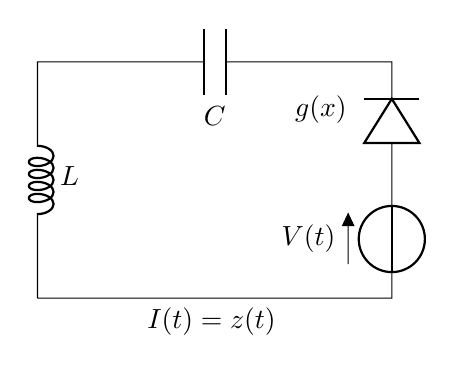
\begin{tikzpicture}[x=1.5cm]
% \draw[help lines] (0,0) grid (5,3);
% \draw (0,0) 
%     to[L] (0,3) 
%     to (2,3) 
%     to[C=$C$] (3,3)
%     to (5,3)
%     to[diode] (5,0) 
%     to (0,0);
%     to[V,v=$U_q$] (0,2) % The voltage source
\draw (0,0) 
    to (3,0)
    to[V,v=$V(t)$] (3,1.5) % The voltage source
    to[diode] (3,3) 
    to (3,3)
    to[C=$C$] (0,3)
%     to (0,3)
    to[L=$L$](0,0) 
    to (0,0);
    % \draw (2,0) to[C] (2,3);
% \draw (3,0) to[C] (3,3);
% \draw (2.5,0) node[ground] {};
\draw (2.7,2.7) node[anchor=north east,align=right] {$g(x)$};
\draw (2.1,0) node[anchor=north east,align=right] {$I(t)=z(t)$};
% \draw (1.8,1.5) node[anchor=north east] {$C_1$};
% \draw (2.8,1.5) node[anchor=north east] {$C_2$};
% \draw (-0.2,1.5) node[anchor=north east] {$L$};
\end{tikzpicture}

 
\end{document}

\caption{LC Schaltkreis Diagramm}
\label{fig:lcDiode}
\end{figure}
Das beschreibende System von ODEs hat die Form
\[
 \begin{pmatrix}
  \dot x_1\\
  \dot x_2\\
  \dot x_3\\
 \end{pmatrix}
 = 
 \begin{pmatrix}
  1\\
  x_3\\
  -\left(x_2-CV(x_1) + g(Cx_3)\right)\frac{1}{LC}
 \end{pmatrix}
\]
wobei $x_1$ die Zeit, $x_2$ die Ladung des Kondensators $C$ und $x_3$ die elektrische Stromstärke bezeichnet. Die Spannungsquelle wird mittels $V(t)=\sin(\omega t)$ simuliert und $g(z)$ modelliert mittels der stückweisen linearen Funktion 
\begin{equation}
 g(z) = \frac{z+|z|}{2\alpha} + \frac{z-|z|}{2\beta}  = \begin{cases}
                                                         \frac{z}{\alpha} & z\geq 0\\
                                                         \frac{z}{\beta}  & z<0
                                                        \end{cases}
\label{eq:lcOde}                                                       
\end{equation}
die Diode. Als Konstanten werden ähnliche Werte wie in echten Schaltkreisen verwendet
\[
 L= 10^{-6},~ C=10^{-13},~ \omega = 3\cdot 10^{9},~\alpha = 2,~\beta = 10^{-5}
\]
Als Anfangswert liegt kein Strom an, d.h. $x_1(0)  = x_2(0) = x_3(0) = 0$.

Im Gegensatz zu dem Rolling Stones Beispiel lässt sich dieses Problem nicht in einer Abs-Normal Form darstellen lässt, da es kein stückweise lineares Problem ist. Die in Theorem \ref{thm:quadrApproxPL} besagte Konvergenz zweiter Ordnung ist nun hier zu beachten, da sich das Modell nicht exakt Linearisieren lässt. Als weiteres numerisches Problem stellen sich die kleinen Konstanten $L,C$ und $\beta$ heraus, ebenso wie die kleine Schrittweite in einem Intervall von $[0, 10^{-8}]$. In der Lösung erhalten wir für die Ladung des Kondensators Größenordnungen von $10^{-13}$, welche an der Maschinengenauigkeit von $\approx 1.1\cdot 10^{-16}$ (double precision) grenzen.

\subsection{Lösen der ODE}
\begin{figure}[H]
\footnotesize 
\centering
\begin{minipage}[b]{0.49\linewidth}
% \begin{minipage}[t][3cm][t]{5cm}
\documentclass{standalone}
\usepackage{pgfplots,pgfplotstable}
\IfStandalone{
	\usepackage{pgfplots,pgfplotstable}
	\usetikzlibrary{external}
	\newcommand{\fromRoot}[1]{../#1}
}{%
}
\begin{document}
\tikzsetnextfilename{lc_solution}
\begin{tikzpicture}
\begin{axis}[
	width=\linewidth,
	legend entries ={$Q(t)$},
	xmin=-1E-12,
	xmax=1.5E-8,
	ymin=-1E-16,
 	ymax=2E-13,
 	xlabel=$x_1$,
 	ylabel=$x_2$
]
	%\addplot[mark=none,blue,dashed] table[x=t,y=x]{grad.dat};
% 	\addplot[mark=none,red,very thin] table[x=t,y=x]{j.dat};
% 	 \addplot[blue,very thin] table[x index=0,y index=2] {dat/sol.dat};
 \addplot[blue] table[x index=0,y index=2] {\fromRoot img/data/lc_solution.dat};
\end{axis}
\end{tikzpicture}
\end{document}
\caption*{(a) Ladung des Kondensators}
\end{minipage}
% \quad
\begin{minipage}[b]{0.49\linewidth}
% \begin{minipage}[t][3cm][t]{5cm}
\documentclass{standalone}
\usepackage{pgfplots,pgfplotstable}
\IfStandalone{
	\usepackage{pgfplots,pgfplotstable}
	\usetikzlibrary{external}
	\newcommand{\fromRoot}[1]{../#1}
}{%
}
\begin{document}
\tikzsetnextfilename{lc_solution2}

\begin{tikzpicture}
\begin{axis}[
	width=\linewidth,
	legend entries ={$I(t)$},
	xmin=-1E-12,
	xmax=1.5E-8,
	ymin=-5E-5,
 	ymax=3E-4,
 	xlabel=$x_1$,
 	ylabel=$x_3$
]
	%\addplot[mark=none,blue,dashed] table[x=t,y=x]{grad.dat};
% 	\addplot[mark=none,red,very thin] table[x=t,y=x]{j.dat};
	 \addplot[red,very thin] table[x index=0,y index=3] {\fromRoot img/data/lc_solution.dat};

\end{axis}
\end{tikzpicture}
\end{document}
\caption*{(b) Stromstärke}
\end{minipage}
\caption{LC-Diode Lösung der ODE}
\label{fig:lc_solution}
\end{figure}
Die Lösung der ODEs \eqref{eq:lcOde} wird in Bild \ref{fig:lc_solution} gezeigt. Zu sehen ist, dass der Kondensator sich initial in einem Zyklus auflädt und sich über die Zeit nach und nach entlädt und schließlich in einem periodischen Verhalten mündet. Die Trajektorie der Stromstärke ändert ihr Verhalten mit ihrem Vorzeichen. Desweiteren war es für die Implementierung notwendig, Abbruchtoleranzen von $10^{-14}$ zu wählen. 

\begin{figure}
\centering
\documentclass{standalone}
\IfStandalone{
	\usepackage{pgfplots,pgfplotstable}
	\usetikzlibrary{external}
	\newcommand{\fromRoot}[1]{../#1}
}{%
}
\begin{document}
\tikzsetnextfilename{lc_convergence}
\begin{tikzpicture}
\begin{loglogaxis}[
% 	width=10cm,
	width=\linewidth,
	xlabel=Anzahl der Freiheitsgrade $N$,
% 	ylabel=Fehler in zum Zeitpunkt $T$,
	ymin=1E-13,
 	ymax=4E-7,
	legend entries ={Expl. MP,
	IMP,
	GIMP, 
	},
	legend style={at={(0.5,1.0)},anchor=south},
	legend columns=3
]
  	\addplot[mark=none,red,very thin] table[x index=0,y index=3] {\fromRoot img/data/lc_convergence.dat};%expl midpoint
 	\addplot[mark=none,green,very thin] table[x index=0,y index=2] {\fromRoot img/data/lc_convergence.dat};%impl midpoint
	\addplot[mark=none,blue,very thin] table[x index=0,y index=1] {\fromRoot img/data/lc_convergence.dat};%gen midpoint

	\addplot[mark=none,very thin,gray, yshift=-20pt] 
		table[y={create col/linear regression={x=0,y=1}}] {\fromRoot img/data/lc_convergence.dat}
		  coordinate [pos=0.5] (A)
		  coordinate [pos=0.6] (B)
		;
	% save the slope parameter:
	\pgfmathparse{-\pgfplotstableregressiona}	
	\pgfmathsetmacro{\slope}{\pgfmathresult}
	
	% draw the opposite and adjacent sides
	% of the triangle
	\draw[very thin,gray] (B) -| (A)
	node [pos=0.2,anchor=north]
	{\pgfmathprintnumber{\slope}};
\end{loglogaxis}
\end{tikzpicture}
\end{document}
\caption{Konvergenz LC Diode im Intervall $[0,1.5\cdot 10^{-8}]$ mit $x_0=(0,0,0)$}
\label{fig:lcConvergence}
\end{figure}
Im Konvergenzgraph \ref{fig:lcConvergence} ist ein ähnliches Verhalten wie beim Rolling Stones Beispiel zu erkennen. Nachdem sich der Konvergenzgraph bis ca. $5\cdot 10^2$ Schritten ähnlich wie die implizite Mittelpunktsregel verhält, konvergiert er stabil mit Ordnung 2, während die Implizite Mittelpunktsregel bedingt durch die wenigen Kinks ebenfalls springt. Das Explizite Verfahren konvergiert unterhalb von $10^3$ Schritten nicht. 
Herauszustellen ist also, dass unsere Methoden selbst für nicht stückweise affine Beispiele stabile Konvergenzresultate erzielen.

Die Romberg Extrapolation gestaltet sich in diesem Beispiel schwierig. Zwar ist in Bild \ref{fig:lcRomberg} ein besseres Verhalten der Extrapolation für die GIMP zu erkennen, diese stößt jedoch an die Grenzen sobald sie sich der Maschinengenauigkeit nähert.  Die Konvergenzgeschwindigkeit betrug in diesem Beispiel nur $2.24$. Insbesondere im Abschnitt zwischen $2\cdot 10^{3}$ und $10^4$ ist jedoch eine deutlich exaktere Extrapolation der GIMP im Gegensatz zur Extrapolation der IMP zu beobachten. In diesem Intervall beträgt die Konvergenzgeschwindigkeit jedoch schon $3.89$. 
\begin{figure}[H]
\footnotesize 
\centering
\begin{minipage}[b]{0.49\linewidth}
% \begin{minipage}[t][3cm][t]{5cm}
\documentclass{standalone}
\IfStandalone{
	\usepackage{pgfplots,pgfplotstable}
	\usetikzlibrary{external}
	\newcommand{\fromRoot}[1]{../#1}
}{%
}
\begin{document}
\tikzsetnextfilename{lc_romberg}
\begin{tikzpicture}
\begin{loglogaxis}[
	width=\linewidth,
	xlabel=Anzahl der Freiheitsgrade $N$,
	ylabel=Fehler in zum Zeitpunkt $T$,
% 	ymin=1E-13,
%  	ymax=4E-7,
	legend entries ={
% 	Expl. MP,
	IMP,
	GIMP, 
	Rom IMP,
	Rom GIMP
	},
	legend style={at={(0.5,1.0)},anchor=south},
	legend columns=2
]
  	\addplot[mark=none,green,very thin] table[x index=0,y index=2] {\fromRoot img/data/lc_romberg.dat};%oimpl midpoint
 	\addplot[mark=none,blue,very thin] table[x index=0,y index=1] {\fromRoot img/data/lc_romberg.dat};%gimp midpoint
	\addplot[mark=none,lime,very thin] table[x index=0,y index=5] {\fromRoot img/data/lc_romberg.dat};%rom gen midpoint
	\addplot[mark=none,cyan,very thin] table[x index=0,y index=4] {\fromRoot img/data/lc_romberg.dat};%rom impl midpoint
	
	\addplot[mark=none,very thin,gray, yshift=-20pt] 
		table[y={create col/linear regression={x=0,y=4}}] {\fromRoot img/data/lc_romberg.dat}
		  coordinate [pos=0.5] (A)
		  coordinate [pos=0.6] (B)
		;
	% save the slope parameter:
	\pgfmathparse{-\pgfplotstableregressiona}	
	\pgfmathsetmacro{\slope}{\pgfmathresult}
	
	% draw the opposite and adjacent sides
	% of the triangle
	\draw[very thin,gray] (B) -| (A)
	node [pos=0.2,anchor=north]
	{\pgfmathprintnumber{\slope}};
\end{loglogaxis}
\end{tikzpicture}
\end{document}
\caption*{(a) Gesamt}
\end{minipage}
% \quad
\begin{minipage}[b]{0.49\linewidth}
% \begin{minipage}[t][3cm][t]{5cm}
\documentclass{standalone}
\IfStandalone{
	\usepackage{pgfplots,pgfplotstable}
	\usetikzlibrary{external}
	\newcommand{\fromRoot}[1]{../#1}
}{%
}
\begin{document}
\tikzsetnextfilename{lc_romberg2}
\begin{tikzpicture}
\begin{loglogaxis}[
	width=\linewidth,
	xlabel=Anzahl der Freiheitsgrade $N$,
	ylabel=Fehler in zum Zeitpunkt $T$,
% 	ymin=1E-13,
%  	ymax=4E-7,
	legend entries ={
% 	Expl. MP,
	IMP,
	GIMP, 
	Rom IMP,
	Rom GIMP
	},
	legend style={at={(0.5,1.0)},anchor=south},
	legend columns=2
]
  	\addplot[mark=none,green,very thin] table[x index=0,y index=2] {\fromRoot img/data/lc_romberg2.dat};%oimpl midpoint
 	\addplot[mark=none,blue,very thin] table[x index=0,y index=1] {\fromRoot img/data/lc_romberg2.dat};%gimp midpoint
	\addplot[mark=none,lime,very thin] table[x index=0,y index=5] {\fromRoot img/data/lc_romberg2.dat};%rom gen midpoint
	\addplot[mark=none,cyan,very thin] table[x index=0,y index=4] {\fromRoot img/data/lc_romberg2.dat};%rom impl midpoint
	
	\addplot[mark=none,very thin,gray, yshift=-20pt] 
		table[y={create col/linear regression={x=0,y=4}}] {\fromRoot img/data/lc_romberg2.dat}
		  coordinate [pos=0.5] (A)
		  coordinate [pos=0.6] (B)
		;
	% save the slope parameter:
	\pgfmathparse{-\pgfplotstableregressiona}	
	\pgfmathsetmacro{\slope}{\pgfmathresult}
	
	% draw the opposite and adjacent sides
	% of the triangle
	\draw[very thin,gray] (B) -| (A)
	node [pos=0.2,anchor=north]
	{\pgfmathprintnumber{\slope}};
\end{loglogaxis}
\end{tikzpicture}
\end{document}
\caption*{(b) Ausschnitt}
\end{minipage}
\caption{Romberg Extrapolation}
\label{fig:lcRomberg}
\end{figure}



Beim Fehler über die Zeit ist genau zu erkennen, dass der Fehler sich an den Kinks erhöht. Die GIMP hat gegenüber den anderen Methoden den kleinsten Fehler. 
\begin{figure}[H]
\footnotesize 
\centering
\begin{minipage}[b]{0.49\linewidth}
% \begin{minipage}[t][3cm][t]{5cm}
\documentclass{standalone}
\IfStandalone{
	\usepackage{pgfplots,pgfplotstable}
	\usetikzlibrary{external}
	\newcommand{\fromRoot}[1]{../#1}
}{%
}
\begin{document}
\tikzsetnextfilename{lc_error_over_time}
\begin{tikzpicture}
\begin{axis}[
	width=\linewidth,
	xlabel=Zeitpunkt $t$,
	ylabel=Fehler zum Zeitpunkt $t$,
	legend entries ={Expl. MP,
	IMP,
	GIMP 
	},
% 	legend style={at={(0,1)},anchor=north west}
	legend style={at={(1,1.0)},anchor=south east},
	legend columns=2
]
\addplot[mark=none,red,very thin] table[x index=0,y index=3] {\fromRoot img/data/lc_eot.dat};
\addplot[mark=none,green,very thin] table[x index=0,y index=2] {\fromRoot img/data/lc_eot.dat};
\addplot[mark=none,blue,very thin] table[x index=0,y index=1] {\fromRoot img/data/lc_eot.dat};

\end{axis}
\end{tikzpicture}
\end{document}
\caption*{(a) Am Zeitpunkt $t$}
\end{minipage}
% \quad
\begin{minipage}[b]{0.49\linewidth}
% \begin{minipage}[t][3cm][t]{5cm}
\documentclass{standalone}
\IfStandalone{
	\usepackage{pgfplots,pgfplotstable}
	\usetikzlibrary{external}
	\newcommand{\fromRoot}[1]{../#1}
}{%
}
\begin{document}
\tikzsetnextfilename{lc_error_over_time_all}
\begin{tikzpicture}
\begin{axis}[
	width=\linewidth,
	xlabel=Zeitpunkt $t$,
	ylabel=Fehler zum Zeitpunkt $t$,
	legend entries ={Expl. MP,
	IMP,
	GIMP 
	},
% 	legend style={at={(0,1)},anchor=north west}
	legend style={at={(1,1.0)},anchor=south east},
	legend columns=2,
	xmin=-1E-12,
	xmax=1.5E-8
]
\addplot[mark=none,red,very thin] table[x index=0,y index=3] {\fromRoot img/data/lc_eot_all.dat};
\addplot[mark=none,green,very thin] table[x index=0,y index=2] {\fromRoot img/data/lc_eot_all.dat};
\addplot[mark=none,blue,very thin] table[x index=0,y index=1] {\fromRoot img/data/lc_eot_all.dat};

\end{axis}
\end{tikzpicture}
\end{document}
\caption*{(b) Summiert}
\end{minipage}
\caption{LC Fehler über Zeit mit $N =1024 ,x_0 = [0,0,0]$}
\end{figure}
\subsection{Gradient und Optimierung}
In diesem Abschnitt werden wir die Lösung im Intervall $[0,10^{-8}]$ mit den Anfangswerten $x_0=(0,0,0)$ als Observierungsparameter benutzen. Da wir keine analytische Lösung berechnen können, wird eine Lösung mit einer erheblich exakteren Schrittweite ($4N$) als Vergleichswert verwendet.

Wie in Bild \ref{fig:lcAdjointConvergence} zu erkennen, konvergiert der Gradient bei der LC-Diode mit einer deutlich höheren Ordnung als im Rolling Stones Beispiel. Mit glatten Observierungsparametern ist der mit der GIMP berechnete Gradient von Anfang an zwei Größenordnungen genauer (Bild \ref{fig:lcAdjointConvergence}(b)), als der mit der IMP berechnete Gradient. 
\begin{figure}[H]
\footnotesize 
\centering
\begin{minipage}[b]{0.49\linewidth}
% \begin{minipage}[t][3cm][t]{5cm}
\documentclass{standalone}
\IfStandalone{
	\usepackage{pgfplots,pgfplotstable}
	\usetikzlibrary{external}
	\newcommand{\fromRoot}[1]{../#1}
}{%
}
\begin{document}
\tikzsetnextfilename{lc_convergence_adjoint_discrete}
\begin{tikzpicture}
\begin{loglogaxis}[
	width=\linewidth,
	xlabel=Anzahl der Freiheitsgrade $N$,
	ylabel=Fehler zu $\nabla J$,
	legend entries ={Expl. MP,
	IMP,
	GIMP 
	},
	ymax=3E-5,
	legend style={at={(0.5,1.0)},anchor=south},
	legend columns=2,
]
	\addplot[mark=none,red,very thin] table[x index=0,y index=3] {\fromRoot img/data/lc_convergence_adjoint_discrete.dat};%expl midpoint
 	\addplot[mark=none,green,very thin] table[x index=0,y index=2] {\fromRoot img/data/lc_convergence_adjoint_discrete.dat};%impl midpoint
	\addplot[mark=none,blue,very thin] table[x index=0,y index=1] {\fromRoot img/data/lc_convergence_adjoint_discrete.dat};%gen midpoint

	\addplot[mark=none,very thin,gray, yshift=-20pt] 
		table[y={create col/linear regression={x=0,y=1}}] {\fromRoot img/data/lc_convergence_adjoint_discrete.dat}
		  coordinate [pos=0.2] (A)
		  coordinate [pos=0.3] (B)
		;
	% save the slope parameter:
	\pgfmathparse{-\pgfplotstableregressiona}	
	\pgfmathsetmacro{\slope}{\pgfmathresult}
	
	% draw the opposite and adjacent sides
	% of the triangle
	\draw[very thin,gray] (B) -| (A)
	node [pos=0.2,anchor=north]
	{\pgfmathprintnumber{\slope}};
\end{loglogaxis}
\end{tikzpicture}
\end{document}
\caption*{(a) Diskrete Observierung}
\end{minipage}
% \quad
\begin{minipage}[b]{0.49\linewidth}
% \begin{minipage}[t][3cm][t]{5cm}
\documentclass{standalone}
\IfStandalone{
	\usepackage{pgfplots,pgfplotstable}
	\usetikzlibrary{external}
	\newcommand{\fromRoot}[1]{../#1}
}{%
}
\begin{document}
\tikzsetnextfilename{lc_convergence_adjoint_smooth}
\begin{tikzpicture}
\begin{loglogaxis}[
	width=\linewidth,
	xlabel=Anzahl der Freiheitsgrade $N$,
	ylabel=Fehler zu $\nabla J$,
	legend entries ={Expl. MP,
	IMP,
	GIMP 
	},
	ymax=3E-5,
	legend style={at={(0.5,1.0)},anchor=south},
	legend columns=2
]
  	\addplot[mark=none,red,very thin] table[x index=0,y index=3] {\fromRoot img/data/lc_convergence_adjoint_smooth.dat};%expl midpoint
 	\addplot[mark=none,green,very thin] table[x index=0,y index=2] {\fromRoot img/data/lc_convergence_adjoint_smooth.dat};%impl midpoint
	\addplot[mark=none,blue,very thin] table[x index=0,y index=1] {\fromRoot img/data/lc_convergence_adjoint_smooth.dat};%gen midpoint

	\addplot[mark=none,very thin,gray, yshift=-20pt] 
		table[y={create col/linear regression={x=0,y=1}}] {\fromRoot img/data/lc_convergence_adjoint_smooth.dat}
		  coordinate [pos=0.2] (A)
		  coordinate [pos=0.3] (B)
		;
	% save the slope parameter:
	\pgfmathparse{-\pgfplotstableregressiona}	
	\pgfmathsetmacro{\slope}{\pgfmathresult}
	
	% draw the opposite and adjacent sides
	% of the triangle
	\draw[very thin,gray] (B) -| (A)
	node [pos=0.2,anchor=north]
	{\pgfmathprintnumber{\slope}};
\end{loglogaxis}
\end{tikzpicture}
\end{document}
\caption*{(b) Glatte Observierung}
\end{minipage}
\caption{LC Diode Konvergenz $\nabla J(x_0)$, \\$I=[0,10^{-8}],x_0=(0,0,10^{-13})$}
\label{fig:lcAdjointConvergence}
\end{figure}

Die Optimierung über das Kostenfunktional, Bild \ref{fig:lcOpt}, verläuft mit der GIMP ebenfalls stabiler als mit der IMP. Man sieht, dass nach zirka 5 Schritten die Konvergenz zunimmt bis sie schließlich nach 19 Schritten konvergiert \ref{fig:lcOpt}(a). Die Berechnung mit der IMP konvergiert nicht so gleichmäßig wie die GIMP. Jedoch ist das Konvergenzverhalten abhängig vom  initiale gewählten Anfangswert. In Bild \ref{fig:lcOpt}(b) konvergieren die IMP und die GIMP fast gleichschnell.

\begin{figure}[H]
\footnotesize
\centering
\begin{minipage}[b]{0.49\linewidth}
% \begin{minipage}[t][3cm][t]{5cm}
\documentclass{standalone}
\usepackage{pgfplots,pgfplotstable}
\IfStandalone{
	\usepackage{pgfplots,pgfplotstable}
	\usetikzlibrary{external}
	\newcommand{\fromRoot}[1]{../#1}
}{%
}
\begin{document}
\tikzsetnextfilename{lc_opt1_convergence}
\begin{tikzpicture}
\begin{axis}[
	width=\linewidth,
	xlabel=Optimierungsschritte,
	ylabel=Fehler,
% 	title=Convergence of Optimization for Rolling Stones,
	legend entries ={IMP,GIMP},
	legend style={at={(0.5,1.0)},anchor=south},
	legend columns=2
]
  	
 	\addplot[mark=none,green,very thin] table[x index=0,y index=2] {\fromRoot img/data/lc_convergence_opt_new.dat};%impl midpoint
	\addplot[mark=none,blue,very thin] table[x index=0,y index=1] {\fromRoot img/data/lc_convergence_opt_new.dat};%gen midpoint
\end{axis}
\end{tikzpicture}

\end{document}
\caption*{(a) $x_0=(0,10^{-10},3\cdot 10^{-8})$}
\end{minipage}
% \quad
\begin{minipage}[b]{0.49\linewidth}
% \begin{minipage}[t][3cm][t]{5cm}
\documentclass{standalone}
\usepackage{pgfplots,pgfplotstable}
\IfStandalone{
	\usepackage{pgfplots,pgfplotstable}
	\usetikzlibrary{external}
	\newcommand{\fromRoot}[1]{../#1}
}{%
}
\begin{document}
\tikzsetnextfilename{lc_opt2_convergence}
\begin{tikzpicture}
\begin{loglogaxis}[
	width=\linewidth,
	xlabel=Optimierungsschritte,
	ylabel=Fehler,
% 	title=Convergence of Optimization for Rolling Stones,
	legend entries ={IMP,GIMP},
	legend style={at={(0.5,1.0)},anchor=south},
	legend columns=2
]
  	
 	\addplot[mark=none,green,very thin] table[x index=0,y index=2] {\fromRoot img/data/lc_opt2_convergence.dat};%impl midpoint
	\addplot[mark=none,blue,very thin] table[x index=0,y index=1] {\fromRoot img/data/lc_opt2_convergence.dat};%gen midpoint
\end{loglogaxis}
\end{tikzpicture}

\end{document}
\caption*{(b) $x_0=(0,10^{-11},5\cdot 10^{-7})$}
\end{minipage}
\caption{LC Diode Data Assimilation Optimierung auf dem Intervall $I = [0,10^{-8}], N=512$}
\label{fig:lcOpt}
\end{figure}


\section{Shallow Water Equation}
% \subsection{Problemstellung}
Bisher wurde die stückweise Linearisierung nur mit gewöhnlichen Differentialgleichungen durchgeführt; Ziel dieses Beispieles ist es, diese Methoden auf eine partielle Differentialgleichungen anzuwenden und an ihr Data Assimilation zu betreiben.

Ein oft genutztes Beispiel, in dem Datenassimilierungsmethoden Anwendung finden ist die sogenannte Shallow Water Equation (vgl. \cite{zou,navon}). 
Diese partiellen Differentialgleichungen gehören zur Klasse der Saint-Venan Systemen und beschreiben eine Strömung einer Flüssigkeit in einem Gebiet unter Berücksichtigung diverser Nebenbedingungen wie Gravitationswellen, Bodenbegebenheit und Randgebiete. Eingeführt wurden sie bereits vor über 140 Jahren von Saint-Venant in \cite{saint1871theorie} und werden zur Simulation von Strömungen in Kanälen und Küstengebieten verwendet.

Im einfachsten eindimensionalen Fall ergibt sich das Saint-Venan System zu 
\begin{equation}
\begin{cases}
 h_t + (hu)_x = 0,\\
 (hu)_t + \left[\frac{(hu)^2}{h} + \frac{g}{2}h^2\right]_x = 0
\end{cases} 
\label{eq:swe}
\end{equation}
wobei $u$ die Geschwindigkeit, $hu$ den Wasserabfluss, $h$ die Höhe und $g=9.81 \sfrac{m}{s^2}$ die Gravitationskonstante bezeichnet.
Die Gleichung \eqref{eq:swe} wird 1-D Shallow Water Equation (SWE) genannt.
Diese kann durch Bodengegebenheiten, Reibung oder konvektiver Beschleunigung erweitert werden.
Eine interessante Eigenschaft dieser Gleichung ist, dass sie glatte stationäre Lösung zulässt, die die Bedingungen
\[
 hu = \text{const}, \quad \frac{u^2}{2}+gh = \text{const}
\]
erfüllen und unglatte stationäre Lösungen. Eine stationäre Lösung ist beispielsweise der "ruhende See"
\[
 u=0, \quad h=\text{const}
\]
Methoden, die diese Lösungen erhalten werden als ausgeglichen (well balanced) bezeichnet. Falls die Höhe des Systems $h \approx 0 $, sich also einem \textit{dry state} nähert, kann sie durch numerische Ungenauigkeiten kleiner Null werden, sodass die Berechnung abbricht, da die Eigenwerte der Jacobimatrix von \eqref{eq:swe} die Form $u\pm \sqrt{gh}$ haben.

Der Grundgedanke zur numerischen Lösung des Problemes besteht darin, die hyperbolische partielle Differentialgleichung \eqref{eq:swe} in ein System von ODEs umzuformen, sodass unsere Methoden darauf angewendet werden können.
Dazu nutzen wir die Finite Volumen Methode, welche unter Anderem von LeVeque in \cite{leveque2002finite} ausführlich behandelt wird. Ähnlich wie Finite Differenzen werden Werte an diskreten Punkten in einem Gitter berechnet. Jedoch wird nicht der Punkt allein betrachtet, sondern die gesamten Gitterzellen, die sogenannten Volumen. In jedem dieser Volumen gilt der Erhaltungssatz für eine Größe; in unserem Beispiel die Höhe und der Wasserabfluss. Eine Veränderung der erhaltenden Größe kann nur durch Ab- oder Hinzufließen über den Rand der Gitterzelle geschehen; dieser wird auch als Flux bezeichnet. Dazu wird der Mittelwert der Erhaltungsgrößen in jeder Zelle berechnet. Damit entsteht eine Gleichung über die Veränderung der Größen in der Zeit, welche durch Löser für gewöhnliche Differentialgleichungen berechnet werden können.
TODO: im LeVeque nachschauen und evtl. mit Theoremen ergänzen!

Kurganov bietet in \cite{kurganov2007second} ein robustes Finite Volumen Schema für die SWE an, die sowohl \textit{well balanced} ist als auch den \textit{dry state} behandelt. Es wurde genutzt, um die gewünschte Ortsdiskretisierung durchzuführen. Im Bild \ref{fig:sweSolution} ist die Lösung von \eqref{eq:swe} über die Zeit dargestellt.

\begin{figure}
 \centering
 \documentclass{standalone}
\usepackage{pgfplots,pgfplotstable}
\IfStandalone{
	\usepackage{pgfplots,pgfplotstable}
	\usetikzlibrary{external}
	\newcommand{\fromRoot}[1]{../#1}
}{%
}
\begin{document}
\tikzsetnextfilename{swe_plot}
\begin{tikzpicture}
\begin{axis}[
   view={-20}{60}, 
   grid=both,
   width=12cm,
    xlabel={Zeit $t$},
    ylabel={Gitter $x$},
    zlabel={$h$},
    ]
\addplot3[surf] file {img/data/swe_plot.dat};
% \addplot3[surf] file {img/data/grad1_gimp.dat};

\end{axis}
\end{tikzpicture}
\end{document}
 \caption{Lösung der 1-D SWE auf $I=[0,300]$, Länge $L=500,~\Delta x=10,~\Delta t=1$, periodischen Randbedingungen und normalverteiltem Anfangswert}
 \label{fig:sweSolution}
\end{figure}

% \cite{evans1998partial}
\subsection{FVM Schema und Unglattheiten}
\label{sec:fvmFluxEigen}
Das Schema von Kurganov aus \cite{kurganov2007second} benutzt ein uniformes Gitter mit $x_\alpha=\alpha\cdot \Delta x$ wobei $\Delta x$ den Abstand zum nächsten Gitterpunkt beschreibt. Das Intervall $I_j = [x_{j-\sfrac{1}{2}},x_{j+\sfrac{1}{2}}]$ sei die $j-$te finite Volumenzelle.
Eine zentrale Upwinding Semidiskretisierung von \eqref{eq:swe} ist das folgende System von ODEs
\[
 \frac{d}{dt} \bar U_j = - \frac{H_{j+\sfrac{1}{2}}-H_{j-\sfrac{1}{2}}}{\Delta x}
\]
wobei 
\[
 \bar U_j \approx \frac{1}{\Delta x}\int_{I_j} U(x,t) dx, \quad U:=(h,hu)^\tr
\]
den Mittelwert der Erhaltungsgrößen der j-ten Zelle beschreibt. Der numerische Fluss $H_{j+\sfrac{1}{2}}$ ist definiert als
\[
\begin{aligned}
 H_{j+\sfrac{1}{2}}(t) =& \frac{a^+_{j+\sfrac{1}{2}}F(U^-_{j+\sfrac{1}{2}}) - a^-_{j+\sfrac{1}{2}}F(U^+_{j+\sfrac{1}{2}})}{a^+_{j+\sfrac{1}{2}} -a^-_{j+\sfrac{1}{2}}} \\
 & +\frac{a^+_{j+\sfrac{1}{2}} \cdot a^-_{j+\sfrac{1}{2}}}{a^+_{j+\sfrac{1}{2}} -a^-_{j+\sfrac{1}{2}}}\left[U^+_{j+\sfrac{1}{2}} - U^-_{j+\sfrac{1}{2}}\right]
\end{aligned}
 \]
$F$ beschreibt die eigentliche rechte Seite der PDE
\[
 F(U) := \left( hu, \frac{(hu)^2}{h}  +\frac{g}{2} h^2 \right)^\tr
\]
und $U^\pm_{j+\sfrac{1}{2}}$ sind die linken/rechten Seiten einer Stückweise linearen Rekonstruktion von $U$ zum Zeitpunkt $t$
\[
 U^\pm_{j+\sfrac{1}{2}} = U_{j+\sfrac{1}{2} \pm \sfrac{1}{2}} + \frac{\Delta x}{2} \left(U_x\right)_{j+\sfrac{1}{2}\pm\sfrac{1}{2}}
\]
Die numerischen Ableitungen $(U_x)_j$ sind die Komponentenweisen Approximationen von $U_x(x_j ,t)$, welche durch nichtlineare \textit{Flux Limiter} berechnet werden, 
da ansonsten oszillatorischen Verhalten in der Lösung auftreten kann aufgrund von zu starken Änderungen der Steigung.(TODO: RAUSSUCHEN WO DAS STEHT).
Der verallgemeinerte MinMod Flux Limiter wurde in der Implementierung benutzt und hat die Form
\[
 \left(U_x\right) = \text{minmod}\left(\theta \frac{\bar U_j- \bar U_{j-1}}{\Delta x},\frac{\bar U_{j+1}- \bar U_{j-1}}{2\Delta x},\theta\frac{ \bar U_{j+1}- \bar U_{j}}{\Delta x}  \right), \quad \theta \in [1,2]
\]
wobei minmod definiert ist als
\[
 \text{minmod}(z_1,z_2,\ldots) = \begin{cases}
                                  \min_j z_j & \text{falls }z_j>0~\forall j\\
                                  \max_j z_j & \text{falls }z_j<0~\forall j\\
                                  0 & \text{sonst}
                                 \end{cases}
 \]
 TODO: LITERATUR MIT ANGEBEN
Diesen kann man in max - min Repräsentation überführen, sodass wir die Funktion
 \begin{equation}
\text{minmod}(z_1,z_2,z_3) = \min(\max(z_1,z_2,z_3),0) + \max(\min(z_1,z_2,z_3),0)    
 \end{equation}

erhalten. Die Konstante $\theta$ wird, falls nicht anders beschrieben, in unseren Beispielen auf $\theta=1$ gesetzt.

Die rechts/linksseitigen lokalen Geschwindigkeiten $a^\pm_{j+\sfrac{1}{2}}$ werden aus dem größten und kleinsten Eigenwert der Jacobimatrix $\frac{\partial F}{\partial U}$ von \eqref{eq:swe} berechnet, wobei sie sich ergeben zu
\[
 \begin{aligned}
 a^+_{j+\sfrac{1}{2}} &= \max \left\lbrace u^+_{j+\sfrac{1}{2}} + \sqrt{gh^+_{j+\sfrac{1}{2}}},u^-_{j+\sfrac{1}{2}} + \sqrt{gh^-_{j+\sfrac{1}{2}}},0\right\rbrace\\
 a^-_{j+\sfrac{1}{2}} &= \max \left\lbrace u^+_{j+\sfrac{1}{2}} - \sqrt{gh^+_{j+\sfrac{1}{2}}},u^-_{j+\sfrac{1}{2}} - \sqrt{gh^-_{j+\sfrac{1}{2}}},0\right\rbrace
 \end{aligned}
\]
mit \begin{equation}
u=\frac{h(hu)}{h^2 + \varepsilon}
\label{eq:sweHuToU}
    \end{equation}
In den numerischen Experimenten ist $\varepsilon = \sfrac{1}{\Delta x^4}$ gewählt.
\begin{figure}
\footnotesize
\centering
\begin{minipage}[b]{\linewidth}
% \begin{minipage}[t][3cm][t]{5cm}
\documentclass{standalone}
\usepackage{pgfplots,pgfplotstable}
\IfStandalone{
	\usepackage{pgfplots,pgfplotstable}
	\usetikzlibrary{external}
	\newcommand{\fromRoot}[1]{../#1}
}{%
}
\begin{document}
\tikzsetnextfilename{swe_grad_3d}
\begin{tikzpicture}
    \begin{axis}[
    view={-20}{60},
    grid=both,
    width=\linewidth,
%      title={$\sfrac{\partial J}{\partial x_0^{(1)}}$},
    xlabel={Zeit $t$},
    ylabel={Ort $x$},
    zlabel={$h_t$}]
      \addplot3[surf] file {\fromRoot img/data/swe_grad_3d.dat};
    \end{axis}
\end{tikzpicture}
\end{document}
\caption*{(a) Höhe RHS}
\end{minipage}
% \quad
\begin{minipage}[b]{0.49\linewidth}
% \begin{minipage}[t][3cm][t]{5cm}
\documentclass{standalone}
\usepackage{pgfplots,pgfplotstable}
\usepackage{ifthen}
\usepackage{intcalc}

\IfStandalone{
	\usepackage{pgfplots,pgfplotstable}
	\usetikzlibrary{external}
	\newcommand{\fromRoot}[1]{../#1}
}{%
}
\begin{document}
\tikzsetnextfilename{swe_grad_rhs_1}
\begin{tikzpicture}
     \begin{axis}[view={-20}{60},
  %  grid=both,
    width=\linewidth,
%     title={Height SWE},
    xlabel={$t$},
%     ymax=0.005,
%     ymin=-0.005,
    ylabel={Rechte Seite},
]
%       \foreach \ind in {0,4,...,61}{
      \foreach \ind in {30,32,...,61}{

	\addplot[mark=none,very thin,blue] table[x index=0,y index=1] {\fromRoot img/data/swe_grad_bundle/gradCut\ind.dat};

% 	  \addplot[mark=none,very thin,red] table[x index=0,y index=1] {dat/gradCut\ind.dat};

      }
    \end{axis}
\end{tikzpicture}
\end{document}
\caption*{(b) Querschnitt Höhe $h$}
\end{minipage}
\begin{minipage}[b]{0.49\linewidth}
% \begin{minipage}[t][3cm][t]{5cm}
\documentclass{standalone}
\usepackage{pgfplots,pgfplotstable}
\usepackage{ifthen}
\usepackage{intcalc}

\IfStandalone{
	\usepackage{pgfplots,pgfplotstable}
	\usetikzlibrary{external}
	\newcommand{\fromRoot}[1]{../#1}
}{%
}
\begin{document}
\tikzsetnextfilename{swe_grad_rhs_2}
\begin{tikzpicture}
     \begin{axis}[view={-20}{60},
  %  grid=both,
    width=\linewidth,
%     title={Height SWE},
%     ymax=0.003,
%     ymin=-0.003,    
    xlabel={$t$},
    ylabel={Rechte Seite},
]
     \foreach \ind in {31,33,...,61}{
%      \foreach \ind in {1,5,...,61}{
%         \ifnum\intcalcMod{\ind}{2}=0
          \addplot[mark=none,very thin,red] table[x index=0,y index=1] {\fromRoot img/data/swe_grad_bundle/gradCut\ind.dat};
      }
    \end{axis}
\end{tikzpicture}
\end{document}
\caption*{(c) Querschnitt Abfluss $hu$}
\end{minipage}
\caption{Rechte Seite der SWE über $I=[0,300], L=300, \Delta x=10, \Delta t = 1$}
\label{fig:sweGrad}
\end{figure}


Die Berechnung der Eigenwerte und der Ableitungen über den MinMod Limiter bringen die Unglattheiten auf der rechten Seite von \eqref{eq:swe}.  Der verallgemeinerte MinMod hat die switching depth $\nu = 3$ und erzeugt dadurch Knicke im computational graph. Ebenso die Eigenwertberechnung, welche eine switching depth von $\nu = 2$ erzeugt. In Figur \ref{fig:sweGrad} ist die Rechte Seite in der Zeit abgebildet. Man kann erkennen, dass Knicke auf der rechten Seite vorhanden sind, die auftreten, falls eine flache in eine steile Steigung übergeht und vice versa. Ebenso ist das oszillatorische Verhalten an den Knicken zu erkennen, welche zu Fehlern in der Zeitintegration mit klassichen Methoden führen.

\subsection{Anfangswerte}
\begin{figure}[H]
\footnotesize
\centering
\begin{minipage}[b]{0.49\linewidth}
% \begin{minipage}[t][3cm][t]{5cm}
\documentclass{standalone}
\IfStandalone{
	\usepackage{pgfplots,pgfplotstable}
	\usetikzlibrary{external}
	\newcommand{\fromRoot}[1]{../#1}
}{%
}
\begin{document}
\tikzsetnextfilename{swe_initial_values}
\begin{tikzpicture}
\begin{axis}[
	width=\linewidth,
% 	grid=both,
	xlabel=$x$,
	ylabel=$h$,
	legend entries ={
	$U_0^{(1)}$,
	$U_0^{(2)}$,
% 	$U_0^{(3)}$,
% 	$U_0^{(4)}$
	},
	legend style={at={(0.5,1.0)},anchor=south},
	legend columns=2
]
      
%       \addplot[mark=none,green,very thin] table[x index=0,y index=2] {\fromRoot img/data/swe_initial_values.dat};%expl midpoint
      \addplot[mark=none,red,very thin] table[x index=0,y index=3] {\fromRoot img/data/swe_initial_values.dat};%expl midpoint
      \addplot[mark=none,blue,very thin] table[x index=0,y index=1] {\fromRoot img/data/swe_initial_values.dat};%expl midpoint
      %       \addplot[mark=none,cyan,very thin] table[x index=0,y index=4] {\fromRoot img/data/swe_initial_values.dat};%expl midpoint
 	\end{axis}
 	%f
\end{tikzpicture}
\end{document}
\caption*{(a) $h$}
\end{minipage}
\begin{minipage}[b]{0.49\linewidth}
% \begin{minipage}[t][3cm][t]{5cm}
\documentclass{standalone}
\IfStandalone{
	\usepackage{pgfplots,pgfplotstable}
	\usetikzlibrary{external}
	\newcommand{\fromRoot}[1]{../#1}
}{%
}
\begin{document}
\tikzsetnextfilename{swe_initial_values_hu}
\begin{tikzpicture}
\begin{axis}[
	width=\linewidth,
% 	grid=both,
	xlabel=$x$,
	ylabel=$hu$,
	legend entries ={
	$U_0^{(1)}$,
	$U_0^{(2)}$,
% 	$x_0^{(3)}$,
% 	$x_0^{(4)}$
	},
	legend style={at={(0.5,1.0)},anchor=south},
	legend columns=2
]
   
%       \addplot[mark=none,green,very thin] table[x index=0,y index=6] {\fromRoot img/data/swe_initial_values.dat};%expl midpoint
      \addplot[mark=none,red,very thin] table[x index=0,y index=7] {\fromRoot img/data/swe_initial_values.dat};%expl midpoint
%       \addplot[mark=none,cyan,very thin] table[x index=0,y index=8] {\fromRoot img/data/swe_initial_values.dat};%expl midpoint
    \addplot[mark=none,blue,very thin] table[x index=0,y index=5] {\fromRoot img/data/swe_initial_values.dat};%expl midpoint
 \end{axis}
 	%tfewfe
\end{tikzpicture}
\end{document}
\caption*{(b) $hu$}
\end{minipage}
\caption{SWE Anfangswerte}
\label{fig:sweInitialValues}
\end{figure}
Die benutzten Anfangswerte $U_0 = (h_0,(hu)_0)$ sind in Bild \ref{fig:sweInitialValues} ersichtlich. Genauer ergeben sie sich zu
\[
\begin{aligned}
 h_0^{(1)} \sim 50\cdot\mathcal N(0.5\cdot L,L) + 1 &&(hu)_0^{(1)}\sim 50\cdot\mathcal N(0.5\cdot L,L) && \text{(Normalverteilt)}\\
 h_0^{(2)}(x)= \sin\left( \frac{2\pi k\cdot x}{L}\right) + 1.5 &&(hu)_0^{(2)}(x) = \cos\left( \frac{2\pi k\cdot x}{L}\right) + 1  && \text{(Schwingung)}
\end{aligned}
\]
Wobei $\mathcal N(\mu, \sigma^2)$ die Normalverteilung mit Erwartungswert $\mu$ und Varianz $\sigma^2$ ist. Falls $U_0^{(2)}$ gewählt wurde ist mit $k\in \R$ die Periode definiert. 
\subsection{Lösen der ODE}
Auch bei der Shallow Water Equation erhalten wir eine Konvergenz von $\mathcal O(\hat h^2)$, mit $\hat h$ als die Schrittweite. Wie im Bild \ref{fig:sweConvergence} ersichtlich, ist der Konvergenzgraph sehr stabil gegenüber der implizitem Mittelpunktsregel, wobei letztere stark springt.

Im Falle einer Schrittweite von $1.6\cdot 10^2$ divergiert die implizite Mittelpunktsregel, wobei die GIMP konvergiert.

Die Romberg Extrapolation konvergiert wie in den vorherigen Beispielen mit einer Ordnung von etwas weniger als $\mathcal O(\hat h^3)$. 

\begin{figure}
\centering
\documentclass{standalone}
\IfStandalone{
	\usepackage{pgfplots,pgfplotstable}
	\usetikzlibrary{external}
	\newcommand{\fromRoot}[1]{../#1}
}{%
}
\begin{document}
\tikzsetnextfilename{swe_convergence}
\begin{tikzpicture}
\begin{loglogaxis}[
	width=\linewidth,
% 	grid=both,
	xlabel=Anzahl der Freiheitsgrade $N$,
	ylabel=Fehler in zum Zeitpunkt $T$,
% 	ymin=1E-13,
%  	ymax=4E-7,
	legend entries ={
	Expl. MP,
	IMP,
	GIMP, 
% 	Rom. GIMP,
% 	Rom. IMP
	},
% 	legend style={at={(0.5,1.0)},anchor=south},
% 	legend columns=2
]
  	\addplot[mark=none,red,very thin] table[x index=0,y index=2] {\fromRoot img/data/swe_convergence.dat};%expl midpoint
 	\addplot[mark=none,green,very thin] table[x index=0,y index=3] {\fromRoot img/data/swe_convergence.dat};%impl midpoint
	\addplot[mark=none,blue,very thin] table[x index=0,y index=1] {\fromRoot img/data/swe_convergence.dat};%gen midpoint
% 	\addplot[mark=none,lime,very thin] table[x index=0,y index=5] {\fromRoot img/data/swe_convergence.dat};%gen midpoint impl
% 	\addplot[mark=none,cyan,very thin] table[x index=0,y index=4] {\fromRoot img/data/swe_convergence.dat};%gen midpoint rom
	\addplot[mark=none,very thin,gray, yshift=-20pt] 
		table[y={create col/linear regression={x=0,y=1}}] {\fromRoot img/data/swe_convergence.dat}
		  coordinate [pos=0.5] (A)
		  coordinate [pos=0.6] (B)
		;
	% save the slope parameter:
	\pgfmathparse{-\pgfplotstableregressiona}	
	\pgfmathsetmacro{\slope}{\pgfmathresult}
	
	% draw the opposite and adjacent sides
	% of the triangle
	\draw[very thin,gray] (B) -| (A)
	node [pos=0.2,anchor=north]
	{\pgfmathprintnumber{\slope}};
\end{loglogaxis}
\end{tikzpicture}
\end{document}
\caption{Konvergenz SWE im Intervall $I = [0,50], L=50, \Delta x=10$ mit $U_0^{(1)}$}
\label{fig:sweConvergence}
\end{figure}

\begin{figure}
\centering
\documentclass{standalone}
\IfStandalone{
	\usepackage{pgfplots,pgfplotstable}
	\usetikzlibrary{external}
	\newcommand{\fromRoot}[1]{../#1}
}{%
}
\begin{document}
\tikzsetnextfilename{swe_convergence_romberg}
\begin{tikzpicture}
\begin{loglogaxis}[
% 	width=9cm,
	width=\linewidth,
% 	grid=both,
	xlabel=Anzahl der Freiheitsgrade $N$,
% 	ylabel=Fehler in zum Zeitpunkt $T$,
% 	ymin=1E-13,
%  	ymax=4E-7,
	legend entries ={
% 	Expl. MP,
	IMP,
	GIMP, 
	Romberg GIMP,
	Romberg IMP
	},
	legend style={at={(0.5,1.0)},anchor=south},
	legend columns=2
]
%   	\addplot[mark=none,red,very thin] table[x index=0,y index=3] {\fromRoot img/data/swe_convergence_romberg.dat};%expl midpoint
 	\addplot[mark=none,green,very thin] table[x index=0,y index=2] {\fromRoot img/data/swe_convergence.dat};%impl midpoint
	\addplot[mark=none,blue,very thin] table[x index=0,y index=1] {\fromRoot img/data/swe_convergence.dat};%gen midpoint
	\addplot[mark=none,lime,very thin] table[x index=0,y index=5] {\fromRoot img/data/swe_convergence.dat};%gen midpoint impl
	\addplot[mark=none,cyan,very thin] table[x index=0,y index=4] {\fromRoot img/data/swe_convergence.dat};%gen midpoint rom
	\addplot[mark=none,very thin,gray, yshift=-20pt] 
		table[y={create col/linear regression={x=0,y=4}}] {\fromRoot img/data/swe_convergence.dat}
		  coordinate [pos=0.5] (A)
		  coordinate [pos=0.6] (B)
		;
	% save the slope parameter:
	\pgfmathparse{-\pgfplotstableregressiona}	
	\pgfmathsetmacro{\slope}{\pgfmathresult}
	
	% draw the opposite and adjacent sides
	% of the triangle
	\draw[very thin,gray] (B) -| (A)
	node [pos=0.2,anchor=north]
	{\pgfmathprintnumber{\slope}};
\end{loglogaxis}
\end{tikzpicture}
\end{document}
\caption{Konvergenz SWE Romberg im Intervall $I = [0,50], L=100, \Delta x=10$ mit $U_0^{(1)}$}
\label{fig:sweConvergenceRomberg}
\end{figure}
Dass die verallgemeinerte Mittelpunktsregel eine bessere Integration liefert ist auch im Bild \ref{fig:sweErrorOverTime} ersichtlich, in dem der Fehler über die Zeit geplottet wurde. Während die GIMP anfangs schlechter integriert, besitzt sie, über einen längeren Zeitraum betrachtet, einen deutlich geringeren Fehler im Gegensatz zu den anderen Methoden.

\begin{figure}
\footnotesize
\begin{minipage}[b]{0.49\linewidth}
% \begin{minipage}[t][3cm][t]{5cm}
\centering
\documentclass{standalone}
\IfStandalone{
	\usepackage{pgfplots,pgfplotstable}
	\usetikzlibrary{external}
	\newcommand{\fromRoot}[1]{../#1}
}{%
}
\begin{document}
\tikzsetnextfilename{swe_error_over_time}
\begin{tikzpicture}
\begin{axis}[
	width=\linewidth,
	xlabel=Zeitpunkt $t$,
	ylabel=Fehler zum Zeitpunkt $t$,
	legend entries ={Expl. MP,
	IMP,
	GIMP 
	},
% 	legend style={at={(0,1)},anchor=north west}
	legend style={at={(1,1.0)},anchor=south east},
	legend columns=2
]
\addplot[mark=none,red,very thin] table[x index=0,y index=3] {\fromRoot img/data/swe_error_over_time.dat};
\addplot[mark=none,green,very thin] table[x index=0,y index=2] {\fromRoot img/data/swe_error_over_time.dat};
\addplot[mark=none,blue,very thin] table[x index=0,y index=1] {\fromRoot img/data/swe_error_over_time.dat};

\end{axis}
\end{tikzpicture}
\end{document}
\caption*{(a) Am Zeitpunk $t$}
\end{minipage}
%  \quad 
\begin{minipage}[b]{0.49\linewidth}
% \begin{minipage}[t][3cm][t]{5cm}
\centering
\documentclass{standalone}
\IfStandalone{
	\usepackage{pgfplots,pgfplotstable}
	\usetikzlibrary{external}
	\newcommand{\fromRoot}[1]{../#1}
}{%
}
\begin{document}
\tikzsetnextfilename{swe_error_over_time_all}
\begin{tikzpicture}
\begin{axis}[
	width=\linewidth,
	xlabel=Zeitpunkt $t$,
	ylabel=Fehler zum Zeitpunkt $t$,
% 	axis y line=right,
% 	every axis y label/.style={at={(current axis.right )},rotate=270},
% 	axis y line*=right,
	ylabel near ticks,
	yticklabel pos=right,	
	legend entries ={Expl. MP,
	IMP,
	GIMP 
	},
% 	legend style={at={(0,1)},anchor=north west}
	legend style={at={(0.5,1.0)},anchor=south},
	legend columns=2
]
\addplot[mark=none,red,very thin] table[x index=0,y index=6] {\fromRoot img/data/swe_error_over_time.dat};
\addplot[mark=none,green,very thin] table[x index=0,y index=5] {\fromRoot img/data/swe_error_over_time.dat};
\addplot[mark=none,blue,very thin] table[x index=0,y index=4] {\fromRoot img/data/swe_error_over_time.dat};

\end{axis}
\end{tikzpicture}
\end{document}
\caption*{(b) Summiert}
\end{minipage}
\caption{SWE Fehler über Zeit mit $L=200,\Delta x=10,h = 1$ und $U_0^{(2)},k=2$}
\label{fig:sweErrorOverTime}
\end{figure}
Da in unserem System keine Reibung auftritt und periodische Randbedingungen haben, müssen die Summe der potentiellen und kinetischen Energie konstant sein. Nun können wir den Energieverlust über die Zeit mittels der Formel \eqref{eq:energyVariation} berechnen. Dabei wird die Höhe $h$ als potentielle und $\frac{1}{2}u^2$ als kinetische Energie betrachtet, wobei $u$ sich aus Formel \eqref{eq:sweHuToU} ergibt. Es entsteht (für $\hat h$ als Schrittweite)
\[
 \hat h \left[\sum_{l=0}^{T/\hat h} \left( h_l + \frac{1}{2} u_l^2 - \left(h_0 + \frac{1}{2} u_0^2\right)\right)^2\right]^{\sfrac{1}{2}}
\]
und als Energiefehler Bild \ref{fig:sweEnergyVariation}.
\begin{figure}
\centering
\documentclass{standalone}
\IfStandalone{
	\usepackage{pgfplots,pgfplotstable}
	\usetikzlibrary{external}
	\newcommand{\fromRoot}[1]{../#1}
}{%
}
\begin{document}
\tikzsetnextfilename{swe_energy_variation}
\begin{tikzpicture}
\begin{loglogaxis}[
	width=10cm,
% 	grid=both,
	xlabel=Anzahl der Freiheitsgrade $N$,
	ylabel=Mittelwert des Energieverlustes $T$,
% 	ymin=1E-13,
%  	ymax=4E-7,
	legend entries ={
	Expl. MP,
	IMP,
	GIMP 
% 	Rom. GIMP,
% 	Rom. IMP
	},
% 	legend style={at={(0.5,1.0)},anchor=south},
% 	legend columns=2
]
  	\addplot[mark=none,red,very thin] table[x index=0,y index=2] {\fromRoot img/data/swe_energy_variation.dat};%expl midpoint
 	\addplot[mark=none,green,very thin] table[x index=0,y index=3] {\fromRoot img/data/swe_energy_variation.dat};%impl midpoint
	\addplot[mark=none,blue,very thin] table[x index=0,y index=1] {\fromRoot img/data/swe_energy_variation.dat};%gen midpoint
	%deufe
\end{loglogaxis}
\end{tikzpicture}
\end{document}
\caption{Energievariation der SWE}
\label{fig:sweEnergyVariation}
\end{figure}
Es ist zu erkennen, dass in diesem Beispiel keine Verbesserung bzgl. des Energievariationsfehlers vorhanden ist.
\subsection{Gradient und Optimierung}

\begin{figure}
\footnotesize
\begin{minipage}[b]{0.49\linewidth}
% \begin{minipage}[t][3cm][t]{5cm}
\centering
\documentclass{standalone}
\IfStandalone{
	\usepackage{pgfplots,pgfplotstable}
	\usetikzlibrary{external}
	\newcommand{\fromRoot}[1]{../#1}
}{%
}
\begin{document}
\tikzsetnextfilename{swe_convergence_adjoint_discrete}
\begin{tikzpicture}
\begin{loglogaxis}[
	width=\linewidth,
	xlabel=Anzahl der Freiheitsgrade $N$,
	ylabel=Fehler zu $\nabla J$,
	legend entries ={Expl. MP,
	IMP,
	GIMP 
	},
% 	ymax=3E-5,
	legend style={at={(0.5,1.0)},anchor=south},
	legend columns=2
]
	\addplot[mark=none,red,very thin] table[x index=0,y index=3] {\fromRoot img/data/swe_convergence_adjoint_discrete.dat};%expl midpoint
 	\addplot[mark=none,green,very thin] table[x index=0,y index=2] {\fromRoot img/data/swe_convergence_adjoint_discrete.dat};%impl midpoint
	\addplot[mark=none,blue,very thin] table[x index=0,y index=1] {\fromRoot img/data/swe_convergence_adjoint_discrete.dat};%gen midpoint

	\addplot[mark=none,very thin,gray, yshift=-20pt] 
		table[y={create col/linear regression={x=0,y=1}}] {\fromRoot img/data/swe_convergence_adjoint_discrete.dat}
		  coordinate [pos=0.2] (A)
		  coordinate [pos=0.3] (B)
		;
	% save the slope parameter:
	\pgfmathparse{-\pgfplotstableregressiona}	
	\pgfmathsetmacro{\slope}{\pgfmathresult}
	
	% draw the opposite and adjacent sides
	% of the triangle
	\draw[very thin,gray] (B) -| (A)
	node [pos=0.2,anchor=north]
	{\pgfmathprintnumber{\slope}};
\end{loglogaxis}
\end{tikzpicture}
\end{document}
\caption*{(a) Am Zeitpunk $t$}
\end{minipage}
%  \quad 
\begin{minipage}[b]{0.49\linewidth}
% \begin{minipage}[t][3cm][t]{5cm}
\centering
\documentclass{standalone}
\IfStandalone{
	\usepackage{pgfplots,pgfplotstable}
	\usetikzlibrary{external}
	\newcommand{\fromRoot}[1]{../#1}
}{%
}
\begin{document}
\tikzsetnextfilename{swe_convergence_adjoint_smooth}
\begin{tikzpicture}
\begin{loglogaxis}[
	width=\linewidth,
	xlabel=Anzahl der Freiheitsgrade $N$,
	ylabel=Fehler zu $\nabla J$,
	legend entries ={Expl. MP,
	IMP,
	GIMP 
	},
% 	ymax=3E-5,
	legend style={at={(0.5,1.0)},anchor=south},
	legend columns=2
]
  	\addplot[mark=none,red,very thin] table[x index=0,y index=2] {\fromRoot img/data/swe_convergence_adjoint_smooth.dat};%expl midpoint
 	\addplot[mark=none,green,very thin] table[x index=0,y index=3] {\fromRoot img/data/swe_convergence_adjoint_smooth.dat};%impl midpoint
	\addplot[mark=none,blue,very thin] table[x index=0,y index=1] {\fromRoot img/data/swe_convergence_adjoint_smooth.dat};%gen midpoint

	\addplot[mark=none,very thin,gray, yshift=-20pt] 
		table[y={create col/linear regression={x=0,y=1}}] {\fromRoot img/data/swe_convergence_adjoint_smooth.dat}
		  coordinate [pos=0.2] (A)
		  coordinate [pos=0.3] (B)
		;
	% save the slope parameter:
	\pgfmathparse{-\pgfplotstableregressiona}	
	\pgfmathsetmacro{\slope}{\pgfmathresult}
	
	% draw the opposite and adjacent sides
	% of the triangle
	\draw[very thin,gray] (B) -| (A)
	node [pos=0.2,anchor=north]
	{\pgfmathprintnumber{\slope}};
\end{loglogaxis}
\end{tikzpicture}
\end{document}
\caption*{(b) Summiert}
\end{minipage}
\caption{SWE Fehler über Zeit mit $L=200,\Delta x=10,h = 1$ und $U_0^{(2)},k=2$}
\label{fig:sweConvergenceAdjoint}
\end{figure}




\chapter{Zusammenfassung und Ausblick}

Im Rahmen dieser Arbeit wurden die bisherigen Konzepte der stückweisen Linearisierung von Griewank et. al. aus \cite{monster} und \cite{plan} erfolgreich auf die Datenassimilierung angewandt.

Dazu wurde zuerst die C++ Klasse \texttt{Plan-C} aus der Diplomarbeit von Boeck \cite{boeck14} verwendet, welche mittels der Abs-Normal Form gewöhnliche Differentialgleichung löst. Diese wurde überarbeitet und erweitert, damit sie performanter mit höherdimensionalen Problemen umgehen kann, etwa durch Sparsematrizen, Parallelisierung und Mikrooptimierungen. Als nächstes wurde aufbauend auf der verallgemeinerten Mittelpunktsregel das inhomogene adjungierte tangent linear model \eqref{eq:genMidpointAdjoint} entwickelt und implementiert, welches Unglattheiten und valley tracing modes mit einbezieht. Dadurch ist es gelungen, den Gradienten des Kostenfunktionals stabiler gegenüber Unglattheiten zu machen, welche in einer besseren Konvergenzgeschwindigkeit in der Optimierung über Kostenfunktionale mündete, sowohl beim Rolling Stone als auch bei der LC-Diode.

Als zweiten Kernpunkt der Arbeit wurden die Methoden der stückweisen Linearisierung zum ersten mal auf eine partielle Differentialgleichung, der 1-D Shallow Water Equation, angewandt, obwohl diese per se ein glattes Problem ist. Unglattheiten entstanden erst durch Flux Limiter und Eigenwertberechnungen des verwendeten Finite Volumen Schemas, welche die Zeitintegration mittels der verallgemeinerten impliziten Mittelpunktsregel jedoch wenig beeinträchtigten. Die Optimierung des Kostenfunktionals ist durch den stabileren Gradienten ebenfalls schneller und stabiler konvergiert.

Zu Verbessern gäbe es bei der aktuellen Implementierung allerhand. Beispielsweise ist die Abs-Normal Form zurzeit ohne sparsity (\cite[S.137 ff.]{griewank2008evaluating}) auf dem AD-Tape gespeichert und muss jedes mal beim Erzeugen der Abs-Normal Form aus einer Funktion vollständig gelesen werden. Dies für \texttt{ADOL-C} zu implementieren und in \texttt{Plan-C} zu ergänzen  würde insbesondere bei der Berechnung der Shallow Water Equation, welche eine sehr große Abs-Normal Form besitzt, aber auch anderen partiellen Differentialgleichungen einen sehr großen Geschwindigkeitsvorteil bieten. 
Desweiteren könnte für partielle Differentialgleichungen mit einem feinen Gitter und dementsprechend vielen ODEs die Tapeerstellung parallelisiert werden. Das heißt, dass für jede ODE ein seperates Tape parallel erstellt und dieses am Ende der Auswertung mit den anderen zusammengeführt wird. Zur Implementierung dieser Technik würde sich der MPI Standard (\cite{mpi}) anbieten. Ebenso wären Aspekte der funktionalen Programmierung hier sicher von Vorteil.

\texttt{Plan-C} mit der Trapezregel aus \cite[S.23 (15)]{monster} zu erweitern und mit ihr Datenassimilierung zu betreiben wäre ein weiterer Punkt.
Ein Vorteil, der sich insbesondere auf die Datenassimilierung bezieht, ist dass die Lösung mittels Trapezregel eine quadratische Spline-Interpolation zweiter Ordnung der analytischen Lösung aller Voraussicht nach zulässt. Diese auf den Projektionsoperator anzuwenden wäre eine Vereinfachung der Berechnung, welche zurzeit mittels kubischer Spline Interpolation durchgeführt wird.

Als nächstes wäre es sicher interessant, die stückweise Linearisierung und der damit verbundenen Datenassimilierung auf andere partielle Differentialgleichungen auszuweiten, wie etwa der 2-D Shallow Water Equation (\cite[\S 3]{kurganov2007second}), der Two-Layer Shallow Water Equation (\cite{kurganov2009central}), Bildrekonstruktionen (\cite{korotaev2008retrieving}) oder realen Wettermodellen wie beispielsweise GFS (\cite{gfs}). 
Ebenfalls wäre es sinnvoll zu beobachten, wie sich die die 1-D Shallow Water Equation für andere als periodische Randbedingungen verhält, ebenso wie für andere Finite Volumen Schemata und/oder anderen Flux-Limitern (\cite{juntasaro2004comparative}).
Desweiteren ließe sich das Bolza Problem \eqref{eq:costfunctional} erweitern, etwas durch zusätzliche Steuerungsparameter und Gewichten. 

Weiterhin wäre es sinnvoll nach einer Möglichkeit zu suchen, das Kostenfunktional stückweise zu linearisieren, sodass die Optimierung über das stückweise lineare Modell durchgeführt werden kann.
Unter der Leitung von Andreas Griewank und Andrea Walther wird zurzeit in Paderborn an einem stückweise linearen Optimierungsalgorithmus gearbeitet (\cite{griewank2014lipschitz}), welcher auf gute Ergebnisse hoffen lässt. 
Dieser nutzt als Optimierungsrichtung $d$ den von Filippov vorgestellten kleinsten Gradienten $short$:
\[
d(x) = \text{short}(0,-\partial F(x)) = \text{argmin} \lbrace \|d\| ~|~ -d \in \partial f(x) \rbrace
\]
Diesen, anstatt dem polynomial escape in die Berechnung des Gradienten und in die Optimierung der Datenassimilierung einzubauen wäre ein erster Schritt diese beiden Routinen zu verbessern.

\begin{frame}[allowframebreaks]
\frametitle{Literatur}
% \bibliographystyle{amsalpha}
\printbibliography
\end{frame}

% All your regular slides
% After your last numbered slide
\appendix
\newcounter{finalframe}
\setcounter{finalframe}{\value{framenumber}}

\begin{frame}
\frametitle{3D und 4D Var. data assimilation}

\begin{block}{3D Var}
 \[J_{3DVar} = \frac{1}{2}(x-x_b)^\tr B^{-1} (x-x_b) +  \frac{1}{2} (C(x) -y)^\tr R^{-1}(C(x) -y)\]
\end{block}
\begin{block}{4D Var}
\[J_{4DVar} = \frac{1}{2}(x-x_b)^\tr B^{-1} (x-x_b) + \frac{1}{2} (C(M_i(x)) -y_i)^\tr R^{-1}(C(M_i(x)) -y_i)\]
\end{block}
\begin{itemize}
\item $x_b$ Hintergrund (vorherige Berechnung, Penalty Parameter)
 \item $B$ Fehler-Kovarianzmatrix des Hintergrundfeldes
 \item $R$ Fehler-Kovarianzmatrix der Observierungen
 \item $M_i$ Modelloperator (überführt $x_0$ nach $x_i$)
\end{itemize}
3D Var betrachtet nur einen Zeitpunkt, 4D eine Zeitspanne (rechenintensiver, \cite{huang2003introduction})
\end{frame}

\begin{frame}
\frametitle{Beispiel: Abs Normal Form Berechnung}
  \begin{block}{Beispiel}
\centering
  $
   \begin{aligned}
    F(x_1,x_2) = \begin{pmatrix}
                  x_1 + |z_1| + |z_3|\\
                  x_2
                 \end{pmatrix}
&& \text{mit} &&\begin{aligned}
        z_1 &= x_1-x_2 \\
        z_2 &= x_2 \\
        z_3 &= x_1-z_2        
       \end{aligned}
   \end{aligned}$
  \end{block}
\[
 \begin{lbmatrix}{1}
  z_1\\
  z_2\\
  z_3\\
  \hline
  y_1\\
  y_2
 \end{lbmatrix}
 =
 \begin{lbmatrix}{1}
  0\\
  0\\
  0\\
  \hline
  0\\
  0
 \end{lbmatrix}
 +
 \begin{lbmatrix}{6}
  1&-1 &\vline&0 &0 &0 \\
  0& 1 &\vline&0 &0 &0 \\
  1&0 &\vline&0 &-1 &0 \\
  \hline
  1&0 &\vline&1 &0 &1 \\
  0&1 &\vline&0 &0 &0 \\
 \end{lbmatrix}
 \begin{lbmatrix}{1}
  x_1\\
  x_2\\
  \hline
  |z_1|\\
  |z_2|\\
  |z_3|
 \end{lbmatrix}
\]
\end{frame}

% \begin{frame}[<+->]
% \frametitle{GIMP Algorithmus}
%  ODE SOLVER ALG
% \end{frame}
\begin{frame}[<+->]
\frametitle{Berechnung der GIMP}
\begin{align}
x_n - x_a &= h \int_{-\frac{1}{2}}^{\frac{1}{2}} F(\xo) + \Delta F(\xo,t(x_n-x_a))dt\\
\iff x_n - x_a -h F(\xo)&= \underbrace{h \int_{-\frac{1}{2}}^{\frac{1}{2}} \Delta F(\xo,t(x_n-x_a))dt}_{r(x_n,x_a)}\\
x_n - x_a -h F(\xo) &= r(x_n,x_a)
\end{align}
\begin{align}
  x_n^{\text{(n)}} - x_a - h (F(\xoold) +\Delta F(\xoold,\xonew - \xoold)) &= r(x_n^{\text{(a)}},x_a)\\
 \iff 2\xonew - 2x_a - h (F(\xoold) +\Delta F(\xoold,\xonew - \xoold)) &= r(x_n^{\text{(a)}},x_a)\\
 \iff  2\xonew -  h (F(\xoold) +\Delta F(\xoold,\xonew - \xoold)) &= r(x_n^{\text{(a)}},x_a) + 2x_a
\end{align}
\[x_n = 2\xo - x_a\]
\end{frame}

\begin{frame}[fragile]
\frametitle{Adjoint Algorithmus}
\algrenewcommand{\algorithmiccomment}[1]{\hfill{\scriptsize #1}}
\begin{algorithmic}[1]
 \Function{calc\_kink\_partial}{$\cx,\hx,\Delta x$}
 	\State $\hat{\tau} \gets 0$,$\check{\tau} \gets 0$, $x_{kink} \gets \cx$
 	\State $\bar{A} \gets 0_{n\times n} $, $\hat{A} \gets 0_{n\times n}$
 	\Repeat
 	  \State $\check{\tau} \gets \check{\tau} + \hat{\tau}, ~ x_{kink} \gets x_{kink} +\check{\tau}\Delta x$
 	  \State $\hat{\tau} \gets \check{\tau} + \Call{critMult}{ x_{kink},\Delta x}$ 		 \Comment{Berechne kritischen Multiplikator}
		\If{$\hat{\tau}>1$} $\hat{\tau}\gets 1$ \EndIf 
 		\State $\xo \gets x_{kink}+0.5\cdot \hat{\tau} \Delta x$	\Comment{Berechne Mittelpunkt zwischen den Kinks}
 	  \State $\frac{\partial F(\rx)}{\partial x} \gets $ gen\_jac($\rx,\Delta x$) \Comment{Berechne $\partial F$ aus der Abs-Normalform}
 	  \State $\bar{A} \gets \bar{A} +  \frac{\partial F(\xo)}{\partial x} \cdot (\hat{\tau} - \check{\tau})$ 
 		\State $\hat{A} \gets \hat{A} +  \frac{\partial F(\rx)}{\partial x} \cdot  \left(\frac{1}{2}(\check{\tau} + \hat{\tau})-0.5\right)$ \Comment{Verschiebe $\tau$ um $-0.5$}
 \Until{$\hat{\tau} \geq 1$	}
 \State \Return $[\bar{A}, \hat{A}]$;
 \EndFunction
 \end{algorithmic}
\end{frame}

\begin{frame}[fragile]
\frametitle{Adjoint Algorithmus}
\algrenewcommand{\algorithmiccomment}[1]{\hfill{\scriptsize #1}}
\begin{algorithmic}[1]
%  \Require $x_{0},t_0,T, h,x_{Obs}, TOL$
 \Function{jac\_data\_assimilation}{$x_{0},t_0,T, h,x_{\text{obs}}, TOL$}
 \State $N = \ceilS{\frac{t_0 - T}{h}}$, $\hat{\bar{x}} \gets 0$ \Comment{Setze Anfangswert}
 \State $x \gets  \Call{solveODE}{x_0,t_0, T,h, TOL};$\Comment{Löse ODE in Vorwärtsrichtung}
 \For{$k\gets$ N-1 to $1$} \Comment{Zeitschritt rückwärts}
 	%\State $\rx \gets \cx - \frac h2 F(\cx)$ \Comment{initialization by half Euler}
 	\State $\rx \gets 0.5(x_k + x_{k-1})$ \Comment{Berechne Mittelpunkt}
 	\State $F(\rx) +\Delta F(\rx;\cdot) \gets$ \Call{Update}{} \Comment{Berechne neue Linearisierung an $\rx$}
 	\State $\Delta x \gets x_{k-1}-x_k$\Comment{Berechne neue Richtung}
 	\State $[\bar{A},\hat{A}] \gets \Call{calc\_kink\_partials}{x_k,x_{k-1},\Delta x}$  \Comment{Berechne $\partial F$}
 	%\Until{$\|\hx - \cx - r - h F(\rx)\|$} < TOL
 	\State{\begin{varwidth}[t]{\linewidth}$\check{\bar{x}} \gets$ Solve( \par
		    \hskip\algorithmicindent $I-\frac{h}{2}\bar{A}^\tr + h \hat{A}^\tr)\check{\bar{x}}=$\par 
		    \hskip\algorithmicindent $ (I+\frac{h}{2}\bar{A}^\tr + h\hat{A}^\tr)\hat{\bar{x}}- hC^\tr(C\rx-\rx_{\text{obs}}))$
		    \end{varwidth}
		    }
 \EndFor
 \State \Return $-\check{\bar{x}}$
 \EndFunction
  \end{algorithmic}
\end{frame}
\begin{frame}[allowframebreaks,fragile]
\frametitle{Polynomial Escape}
\algrenewcommand{\algorithmiccomment}[1]{\hfill{\scriptsize #1}}
\begin{algorithmic}[1]
 \Function{gen\_jac}{$x,\Delta x$}
 	\State $k \gets \max_i\lbrace i~|~\Delta x_i\rbrace$
 	\State $z \gets $calculate\_z($x$)
 	\For{$i=1\ldots s$}\Comment{Berechnung von $\nabla z$}
	  \State $\sigma_i\gets \sign(z_i)$ 
	  \State $\nabla z_{i,1} = Z.row(i)\cdot \Delta x$\Comment{Berechne $Z\Delta x$}
	  \State $\nabla z_{i,j+1} = Z.row(i)\cdot e_j$, für $j=1,\ldots,k-1$
	  \State $\nabla z_{i,j} = Z.row(i)\cdot e_j$, für $j=k+1,\ldots, n$
	  \State $\nabla z.row(i) \mathrel{+}= L_{i,j}\cdot \sigma_j\cdot \nabla z.row(j)$ für $j=1,\ldots, i$\Comment{Berechne $L\Sigma \nabla z$}
	  \State $j\gets 2$
	  \While{$\sigma_i==0$ \&\& $j<s$ }\Comment{Firstsign}
	    \State $\sigma_i \gets \sign(\nabla z_{i,j})$
	    \State $j++$
	  \EndWhile
	\EndFor
	\For{$i=1\ldots n$}\Comment{Berechnung von $\nabla y$}
	  \State $\nabla y_{i,1} = J.row(i)\cdot \Delta x$\Comment{Berechne $J\Delta x$}
	  \State $\nabla y_{i,j+1} = J.row(i)\cdot e_j$, für $j=1,\ldots,k-1$
	  \State $\nabla y_{i,j} = J.row(i)\cdot e_j$, für $j=k+1,\ldots, n$
	  \State $\nabla y.row(i) \mathrel{+}= Y_{i,j}\cdot \sigma_j\cdot \nabla z.row(j)$ für $j=1,\ldots, s$\Comment{Berechne $Y\nabla z$}
	\EndFor
	\For{$j=1\ldots n$}\Comment{Berechnung von $J_\sigma^E\cdot E^{-1}$}
	  \State $\tilde J_{i,j} =\nabla y_{j,i+1}$für $i=1,\ldots,k-1$
	  \State $\tilde J_{i,j} = \nabla y_{j,i} $ für $i=k+1,\ldots,n$
	  \State $\tilde J_{k,j} = \nabla y_{j,1}$
	  \State $\tilde J_{k,j} \mathrel{+}= (\tilde J_{i,j}\Delta x_i) / \Delta x_k$ für $i=1,\ldots,k-1,k+1,\ldots,n$
	\EndFor
	\State $J_\sigma = \tilde J$
 \EndFunction
 \end{algorithmic}
\end{frame}

\begin{frame}
\frametitle{LC Diode Adjungierte Gleichung I}
\begin{minipage}[c]{0.45\textwidth}
\centering
\scalebox{0.9}{\documentclass{standalone}
\IfStandalone{
	\usepackage{pgfplots,pgfplotstable}
	\usetikzlibrary{external}
	\newcommand{\fromRoot}[1]{../#1}
}{%
}

\begin{document}
\tikzsetnextfilename{lc_adjoint_sol3}
\begin{tikzpicture}
\begin{axis}[
	width=\linewidth,
	xlabel=Zeit $t$,
	ylabel=$\dot{\overline{\alpha}}$,
	legend entries ={
	$\overline{\alpha}$,
% 	$\dot{\bar x_2}$
	}
% 	legend style={at={(0.5,1.0)},anchor=south},
% 	legend columns=2
]
  	\addplot[mark=none,green,very thin] table[x index=0,y index=4] {\fromRoot img/data/lc_adjoint_sol.dat};%expl midpoint
%    	\addplot[mark=none,blue,very thin] table[x index=0,y index=5] {\fromRoot img/data/lc_adjoint_sol_grad.dat};%expl midpoint
\end{axis}
\end{tikzpicture}
\end{document}}
\scalebox{0.9}{\documentclass{standalone}
\IfStandalone{
	\usepackage{pgfplots,pgfplotstable}
	\usetikzlibrary{external}
	\newcommand{\fromRoot}[1]{../#1}
}{%
}

\begin{document}
\tikzsetnextfilename{lc_adjoint_sol4}
\begin{tikzpicture}
\begin{axis}[
	width=\linewidth,
	xlabel=Zeit $t$,
	ylabel=$\dot{\overline{\beta}}$,
	legend entries ={
	$\overline \beta$,
% 	$\dot{\bar x_2}$
	}
% 	legend style={at={(0.5,1.0)},anchor=south},
% 	legend columns=2
]
  	\addplot[mark=none,green,very thin] table[x index=0,y index=5] {\fromRoot img/data/lc_adjoint_sol.dat};%expl midpoint
%    	\addplot[mark=none,blue,very thin] table[x index=0,y index=5] {\fromRoot img/data/lc_adjoint_sol_grad.dat};%expl midpoint
\end{axis}
\end{tikzpicture}
\end{document}}
\end{minipage}
\begin{minipage}[c]{0.45\textwidth}
\centering
\scalebox{0.9}{\documentclass{standalone}
\IfStandalone{
	\usepackage{pgfplots,pgfplotstable}
	\usetikzlibrary{external}
	\newcommand{\fromRoot}[1]{../#1}
}{%
}

\begin{document}
\tikzsetnextfilename{lc_adjoint_sol3g}
\begin{tikzpicture}
\begin{axis}[
	width=\linewidth,
	xlabel=Zeit $t$,
	ylabel=$\dot{\overline{\alpha}}$,
	legend entries ={
% 	$\bar x_2$,
	$\dot{\overline{\alpha}}$
	}
% 	legend style={at={(0.5,1.0)},anchor=south},
% 	legend columns=2
]
%   	\addplot[mark=none,green,very thin] table[x index=0,y index=5] {\fromRoot img/data/lc_adjoint_sol.dat};%expl midpoint
   	\addplot[mark=none,blue,very thin] table[x index=0,y index=4] {\fromRoot img/data/lc_adjoint_sol_grad.dat};%expl midpoint
\end{axis}
\end{tikzpicture}
\end{document}}
\scalebox{0.9}{\documentclass{standalone}
\IfStandalone{
	\usepackage{pgfplots,pgfplotstable}
	\usetikzlibrary{external}
	\newcommand{\fromRoot}[1]{../#1}
}{%
}

\begin{document}
\tikzsetnextfilename{lc_adjoint_sol4g}
\begin{tikzpicture}
\begin{axis}[
	width=\linewidth,
	xlabel=Zeit $t$,
	ylabel=$\dot{\overline{\beta}}$,
	legend entries ={
% 	$\bar x_2$,
	$\dot{\overline{\beta}}$
	}
% 	legend style={at={(0.5,1.0)},anchor=south},
% 	legend columns=2
]
%   	\addplot[mark=none,green,very thin] table[x index=0,y index=5] {\fromRoot img/data/lc_adjoint_sol.dat};%expl midpoint
   	\addplot[mark=none,blue,very thin] table[x index=0,y index=5] {\fromRoot img/data/lc_adjoint_sol_grad.dat};%expl midpoint
\end{axis}
\end{tikzpicture}
\end{document}}
\end{minipage}
\end{frame}

\begin{frame}
\frametitle{LC Diode Adjungierte Gleichung II}
\begin{minipage}[c]{0.45\textwidth}
\centering
\scalebox{0.9}{\documentclass{standalone}
\IfStandalone{
	\usepackage{pgfplots,pgfplotstable}
	\usetikzlibrary{external}
	\newcommand{\fromRoot}[1]{../#1}
}{%
}

\begin{document}
\tikzsetnextfilename{lc_adjoint_sol1}
\begin{tikzpicture}
\begin{axis}[
	width=\linewidth,
	xlabel=Zeit $t$,
	ylabel=$\dot{\overline{x_2}}$,
	legend entries ={
	$\overline x_2$
	}
% 	legend style={at={(0.5,1.0)},anchor=south},
% 	legend columns=2
]
  	\addplot[mark=none,green,very thin] table[x index=0,y index=2] {\fromRoot img/data/lc_adjoint_sol.dat};%expl midpoint
%    	\addplot[mark=none,blue,very thin] table[x index=0,y index=5] {\fromRoot img/data/lc_adjoint_sol_grad.dat};%expl midpoint
\end{axis}
\end{tikzpicture}
\end{document}}
\scalebox{0.9}{\documentclass{standalone}
\IfStandalone{
	\usepackage{pgfplots,pgfplotstable}
	\usetikzlibrary{external}
	\newcommand{\fromRoot}[1]{../#1}
}{%
}

\begin{document}
\tikzsetnextfilename{lc_adjoint_sol2}
\begin{tikzpicture}
\begin{axis}[
	width=\linewidth,
	xlabel=Zeit $t$,
	ylabel=$\dot{\overline{x_3}}$,
	legend entries ={
	$\overline{x_3}$,
% 	$\dot{\bar x_2}$
	}
% 	legend style={at={(0.5,1.0)},anchor=south},
% 	legend columns=2
]
  	\addplot[mark=none,green,very thin] table[x index=0,y index=3] {\fromRoot img/data/lc_adjoint_sol.dat};%expl midpoint
%    	\addplot[mark=none,blue,very thin] table[x index=0,y index=5] {\fromRoot img/data/lc_adjoint_sol_grad.dat};%expl midpoint
\end{axis}
\end{tikzpicture}
\end{document}}
\end{minipage}
\begin{minipage}[c]{0.45\textwidth}
\centering
\scalebox{0.9}{\documentclass{standalone}
\IfStandalone{
	\usepackage{pgfplots,pgfplotstable}
	\usetikzlibrary{external}
	\newcommand{\fromRoot}[1]{../#1}
}{%
}

\begin{document}
\tikzsetnextfilename{lc_adjoint_sol1g}
\begin{tikzpicture}
\begin{axis}[
	width=\linewidth,
	xlabel=Zeit $t$,
	ylabel=$\dot{\overline{x_2}}$,
	legend entries ={
% 	$\bar x_2$,
	$\dot{\overline{x_2}}$
	}
% 	legend style={at={(0.5,1.0)},anchor=south},
% 	legend columns=2
]
%   	\addplot[mark=none,green,very thin] table[x index=0,y index=5] {\fromRoot img/data/lc_adjoint_sol.dat};%expl midpoint
   	\addplot[mark=none,blue,very thin] table[x index=0,y index=2] {\fromRoot img/data/lc_adjoint_sol_grad.dat};%expl midpoint
\end{axis}
\end{tikzpicture}
\end{document}}
\scalebox{0.9}{\documentclass{standalone}
\IfStandalone{
	\usepackage{pgfplots,pgfplotstable}
	\usetikzlibrary{external}
	\newcommand{\fromRoot}[1]{../#1}
}{%
}

\begin{document}
\tikzsetnextfilename{lc_adjoint_sol2g}
\begin{tikzpicture}
\begin{axis}[
	width=\linewidth,
	xlabel=Zeit $t$,
	ylabel=$\dot{\overline{x_3}}$,
	legend entries ={
% 	$\bar x_3$,
	$\dot{\overline{x_3}}$
	}
% 	legend style={at={(0.5,1.0)},anchor=south},
% 	legend columns=2
]
%   	\addplot[mark=none,green,very thin] table[x index=0,y index=5] {\fromRoot img/data/lc_adjoint_sol.dat};%expl midpoint
   	\addplot[mark=none,blue,very thin] table[x index=0,y index=3] {\fromRoot img/data/lc_adjoint_sol_grad.dat};%expl midpoint
\end{axis}
\end{tikzpicture}
\end{document}}
\end{minipage}
\end{frame}


\begin{frame}
\frametitle{Adjungierte Gleichung Shallow Water Equation}
\begin{minipage}[c]{0.45\textwidth}
\centering
\scalebox{0.9}{\documentclass{standalone}
\IfStandalone{
	\usepackage{pgfplots,pgfplotstable}
	\usetikzlibrary{external}
	\newcommand{\fromRoot}[1]{../#1}
}{%
}

\begin{document}
\tikzsetnextfilename{swe_adjoint_sol1}
\begin{tikzpicture}
\begin{axis}[
	width=\linewidth,
	xlabel=Zeit $t$,
	ylabel=$\overline{h}$,
	legend entries ={
	$\overline{h}$
	},
% 	legend style={at={(0.5,1.0)},anchor=south},
% 	legend columns=2
]
\foreach \ind in {1,2,...,11}{
  	\addplot[mark=none,green,very thin] table[x index=0,y index=\ind] {\fromRoot img/data/swe_adjoint_sol.dat};%expl midpoint
 }
\end{axis}
\end{tikzpicture}
\end{document}}
\scalebox{0.9}{\documentclass{standalone}
\IfStandalone{
	\usepackage{pgfplots,pgfplotstable}
	\usetikzlibrary{external}
	\newcommand{\fromRoot}[1]{../#1}
}{%
}

\begin{document}
\tikzsetnextfilename{swe_adjoint_sol2}
\begin{tikzpicture}
\begin{axis}[
	width=\linewidth,
	xlabel=Zeit $t$,
	ylabel=$\overline{hu}$,
	legend entries ={
	$\overline{hu}$
	},
% 	legend style={at={(0.5,1.0)},anchor=south},
% 	legend columns=2
]
\foreach \ind in {1,2,...,11}{
  	\addplot[mark=none,green,very thin] table[x index=0,y index=\ind] {\fromRoot img/data/swe_adjoint_sol1.dat};%expl midpoint
 }
\end{axis}
\end{tikzpicture}
\end{document}}
\end{minipage}
\begin{minipage}[c]{0.45\textwidth}
\centering
\scalebox{0.9}{\documentclass{standalone}
\IfStandalone{
	\usepackage{pgfplots,pgfplotstable}
	\usetikzlibrary{external}
	\newcommand{\fromRoot}[1]{../#1}
}{%
}

\begin{document}
\tikzsetnextfilename{swe_adjoint_sol1_grad}
\begin{tikzpicture}
\begin{axis}[
	width=\linewidth,
	xlabel=Zeit $t$,
	ylabel=$\dot{\overline{h}}$,
	legend entries ={
	$\dot{\overline{h}}$
	},
% 	legend style={at={(0.5,1.0)},anchor=south},
% 	legend columns=2
]
\foreach \ind in {1,2,...,11}{
  	\addplot[mark=none,blue,very thin] table[x index=0,y index=\ind] {\fromRoot img/data/swe_adjoint_sol_grad.dat};%expl midpoint
 }
\end{axis}
\end{tikzpicture}
\end{document}}
\scalebox{0.9}{\documentclass{standalone}
\IfStandalone{
	\usepackage{pgfplots,pgfplotstable}
	\usetikzlibrary{external}
	\newcommand{\fromRoot}[1]{../#1}
}{%
}

\begin{document}
\tikzsetnextfilename{swe_adjoint_sol2_grad}
\begin{tikzpicture}
\begin{axis}[
	width=\linewidth,
	xlabel=Zeit $t$,
	ylabel=$\dot{\overline{hu}}$,
	legend entries ={
	$\dot{\overline{hu}}$
	},
% 	legend style={at={(0.5,1.0)},anchor=south},
% 	legend columns=2
]
\foreach \ind in {1,2,...,11}{
  	\addplot[mark=none,blue,very thin] table[x index=0,y index=\ind] {\fromRoot img/data/swe_adjoint_sol1_grad.dat};%expl midpoint
 }
\end{axis}
\end{tikzpicture}
\end{document}}
\end{minipage}
\end{frame}





\begin{frame}
\frametitle{Adjungierte Gleichung Rolling Stones}
\begin{minipage}[c]{0.45\textwidth}
\centering
\scalebox{1.1}{\documentclass{standalone}
\IfStandalone{
	\usepackage{pgfplots,pgfplotstable}
	\usetikzlibrary{external}
	\newcommand{\fromRoot}[1]{../#1}
}{%
}

\begin{document}
\tikzsetnextfilename{rolling_adjoint_sol1}
\begin{tikzpicture}
\begin{axis}[
	width=\linewidth,
	xlabel=Zeit $t$,
	ylabel=$\dot{\bar x}$,
	legend entries ={
	$\bar x_1$,
	$\dot{\bar x}_1$
	},
% 	legend style={at={(0.5,1.0)},anchor=south},
% 	legend columns=2
]
  	
  
  \addplot[mark=none,green,very thin] table[x index=0,y index=1] {\fromRoot img/data/rolling_adjoint_solution.dat};%impl midpoint
  \addplot[mark=none,blue,very thin] table[x index=0,y index=1] {\fromRoot img/data/rolling_adjoint_sol_grad.dat};%expl midpoint
  
\end{axis}
\end{tikzpicture}
\end{document}}
\end{minipage}
\begin{minipage}[c]{0.45\textwidth}
\centering
\scalebox{1.1}{\documentclass{standalone}
\IfStandalone{
	\usepackage{pgfplots,pgfplotstable}
	\pgfplotsset{compat=1.10}
	\usetikzlibrary{external}
	\newcommand{\fromRoot}[1]{../#1}
}{%
}

\begin{document}
\tikzsetnextfilename{rolling_adjoint_sol2}
\begin{tikzpicture}
\begin{axis}[
	width=\linewidth,
	xlabel=Zeit $t$,
	ylabel=$\dot{\bar x}$,
	legend entries ={
	$\bar x_2$,
	$\dot{\bar x}_2$
	},
% 	legend style={at={(0.5,1.0)},anchor=south},
% 	legend columns=2
]
      
	
  \addplot[mark=none,green,very thin] table[x index=0,y index=2] {\fromRoot img/data/rolling_adjoint_solution.dat};%impl midpoint	
%   \addplot[mark=none,blue,very thin] table[x index=0,y index=1] {\fromRoot img/data/rolling_adjoint_sol_grad.dat};%expl midpoint
  \addplot[mark=none,blue,very thin] table[x index=0,y index=2] {\fromRoot img/data/rolling_adjoint_sol_grad.dat};%expl midpoint
  
\end{axis}
\end{tikzpicture}
\end{document}}
\end{minipage}
\end{frame}


% \begin{frame}[<+->]
% \frametitle{Experimente}
% CFL IMAGE
% \end{frame}


\begin{frame}[fragile]
\frametitle{Implementierung}
\cite{openblas}
\cite{armadillo}
\cite{ADOLCmanual}
\cite{boeck14}
\end{frame}

% Backup frames
\setcounter{framenumber}{\value{finalframe}}



\end{document}